% $Id: TopLevel.tex,v 1.1 2008/01/31 18:04:17 dconway Exp $
\chapter{\label{chapter:TopLevel}System Architecture Overview}
\chapauthor{Darrel J. Conway}{Thinking Systems, Inc.}

The purpose of this chapter is to introduce the key architectural elements of GMAT, and to explain
at a high level how they interact to solve mission design problems.  If you are trying to understand
how GMAT works, or if you are refreshing yourself in the basics of the GMAT architecture, this
chapter is where you should start.  After reading this chapter, you should have a high level
understanding of how the components in GMAT interact to perform mission analysis.

The chapter is written so that as you read further, you will obtain a deeper the view into the
system architecture.  We begin by identifying the key system components and grouping them according
to the functions they perform.  These groupings are referred to as ``Packages'' and are used to
provide a framework for the discussion about how GMAT works.

After presenting the functional GMAT's components, we present a high level view of how these
components interact and describe which components interact with each other.  This description
provides an overview of how messages and data flow in the system.  The next level of detail
describes how the architecture handles a simple application there a user open the system, creates a
spacecraft, configures a mission sequence, and runs the mission.

Later chapters build on these materials.  The remainder of this document is organized to take the
package descriptions presented at the start of this chapter, and present the design of the elements
of these packages.  Since the document is structured that way, we'll begin this chapter by examining
the logical packaging of GMAT's components.

\section{\label{section:Packaging}The GMAT System Framework}\index{Packages}

\begin{figure}
\begin{center}
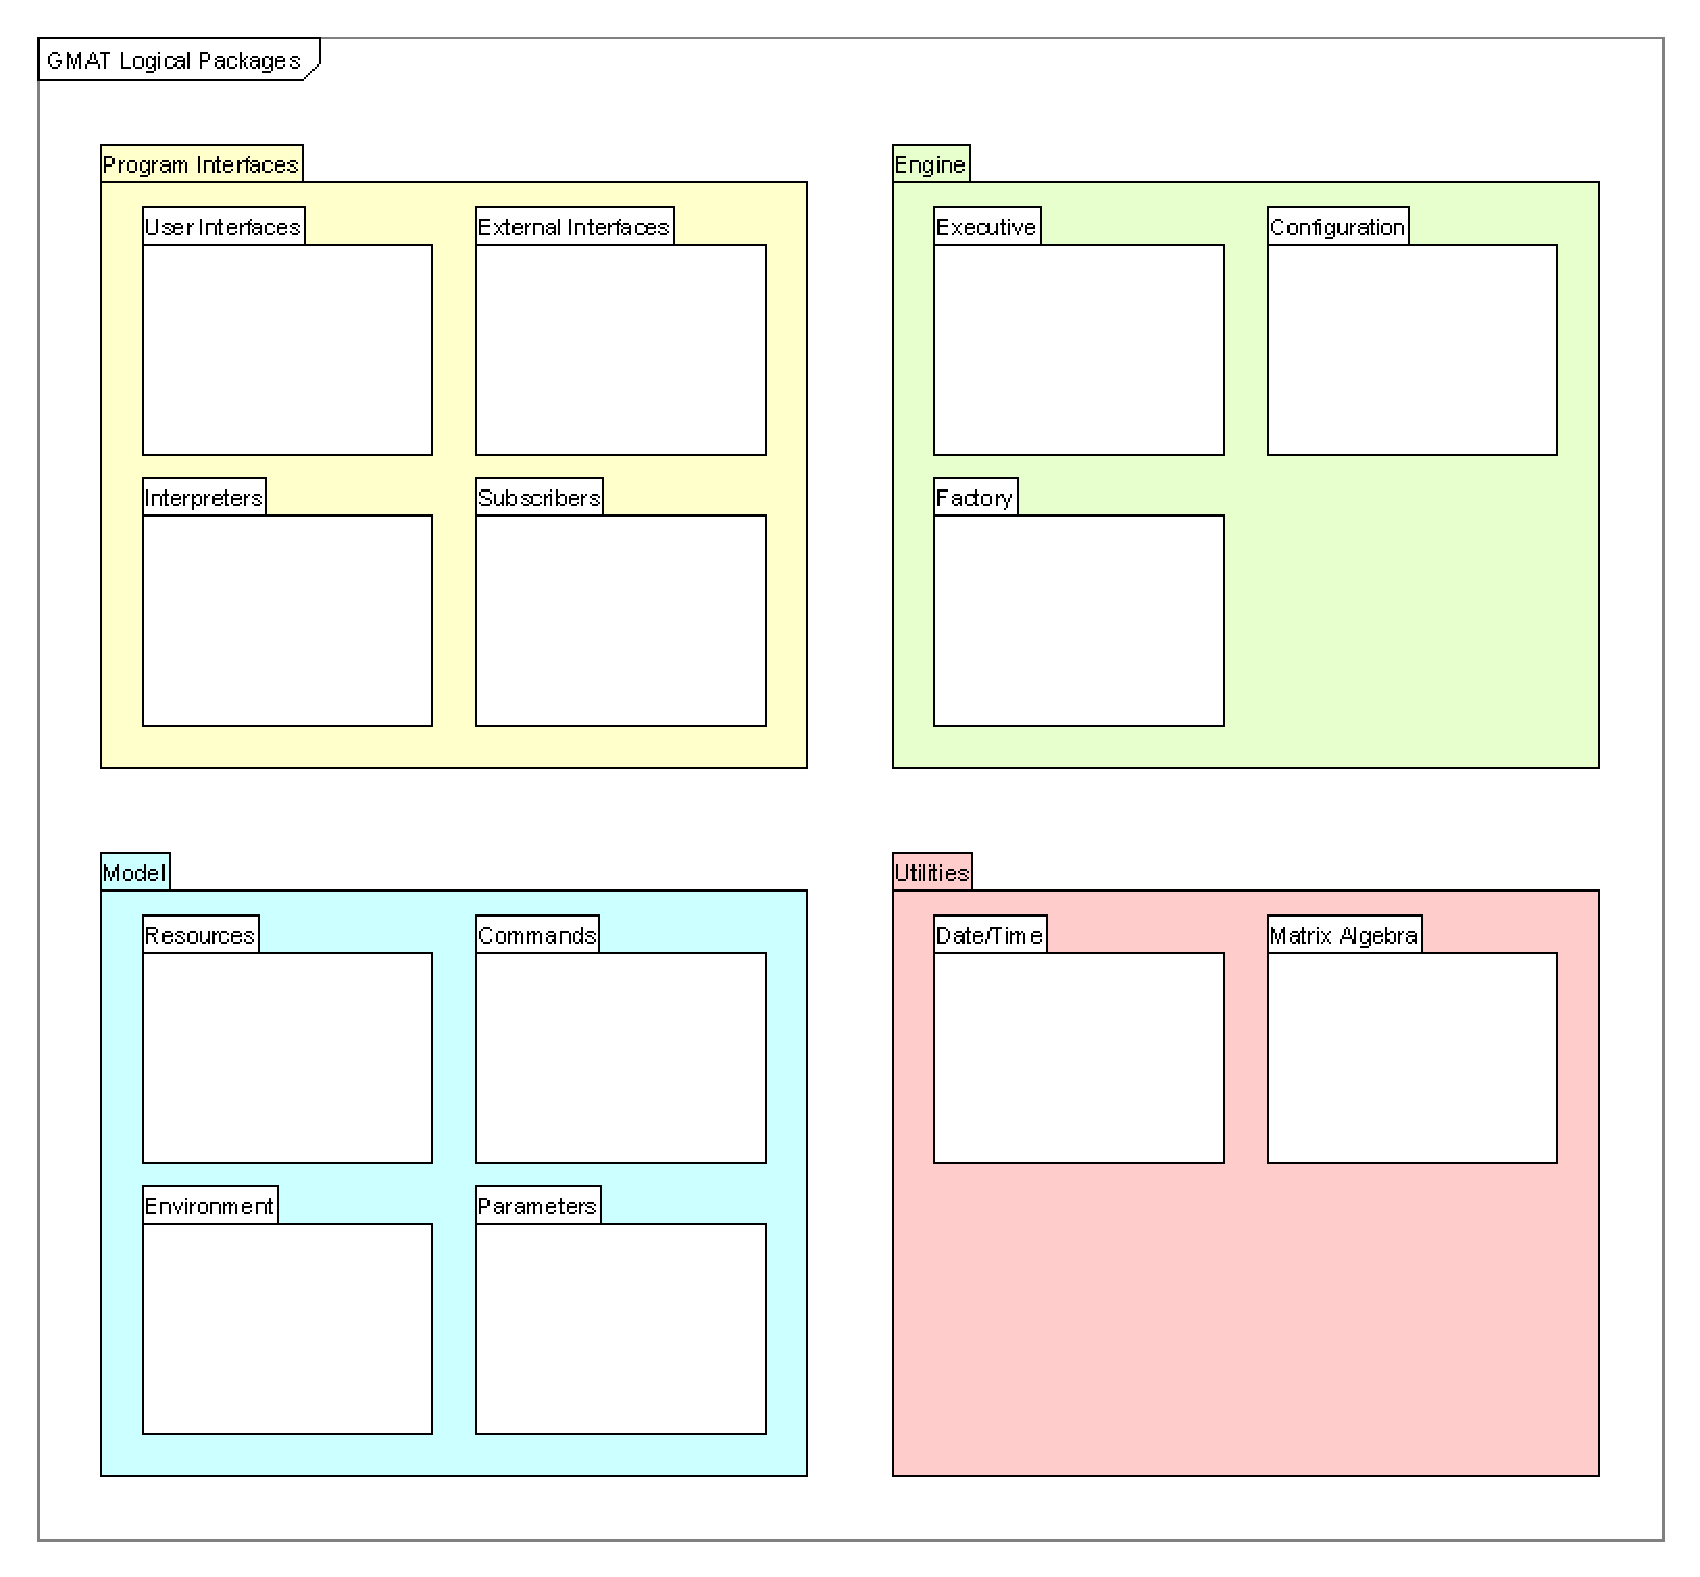
\includegraphics[scale=0.5]{Images/GMATLogicalPackages.eps}
\caption{\label{figure:TopLevelPackages}Top Level GMAT Packages: Logical Grouping}
\end{center}
\end{figure}

% Here is the packaging color scheme used throughout this chapter:
%    Interface package:  pale yellow    RGB: 255 255 153
%    Engine package:     pale green     RGB: 204 255 204
%    Model package:      pale cyan      RGB: 204 255 255
%    Utility package:    pink           RGB: 255 204 204
%    External programs:  pale orange    RGB: 255 204 153
%    GMAT Background:    light grey     RGB: 204 204 204

The GMAT architecture can be described as a set of components grouped into functional
packages\footnote{Note that these divisions are functional, and not enforced by any physical
packaging constraints like a namespace or shared library boundaries.} that interact to model
spacecraft missions.  The system is built around four packages that cooperatively interact to
model spacecraft in orbit. Figure~\ref{figure:TopLevelPackages} shows an overview of this package
grouping.  GMAT functionality can be broken into Program Interfaces, the core system Engine, the
Model used to simulate spacecraft and their environment, and Utilities providing core programmatic
functionality. The constituents of these packages are described throughout this document; this
chapter provides a framework for the more detailed discussions that follow.

Each of these functional categories can be broken into smaller units.  The next level of
decomposition is also shown in Figure~\ref{figure:TopLevelPackages}.  This next level of packaging
-- referred to as ``subpackaging'' in this document -- provides a finer grained view of the
functions provided in each package.  The next level of decomposition below the subpackages
provides a view into the class structure of GMAT, as will be seen in the next few paragraphs.

\subsection{Package and Subpackage Descriptions}

Figure~\ref{figure:PackageHierarchy} presents the packages and subpackages in a slightly different
format from that shown in the last figure.  The top level packages are represented by specific
colors matching those in Figure~\ref{figure:TopLevelPackages}\footnote{This color scheme will be
used for the remainder of this chapter as well.}.  The package names are listed at the top of each
column, with the subpackages shown indented one level from these packages.  One additional level is
shown in this diagram, showing representative members of the subpackages.  The deepest level items
in this figure are classes contained in the subpackages; for example, the Executive subpackage in
the Engine package contains the Moderator, Sandbox, and Publisher classes.  These elements will be
used in the discussion of how the packages interact in the next few pages of this document.

As is shown in these figures, three of these packages can be further broken into subpackages.  The
following paragraphs present an overview of the packages and their subdivisions.

\begin{figure}
\begin{center}
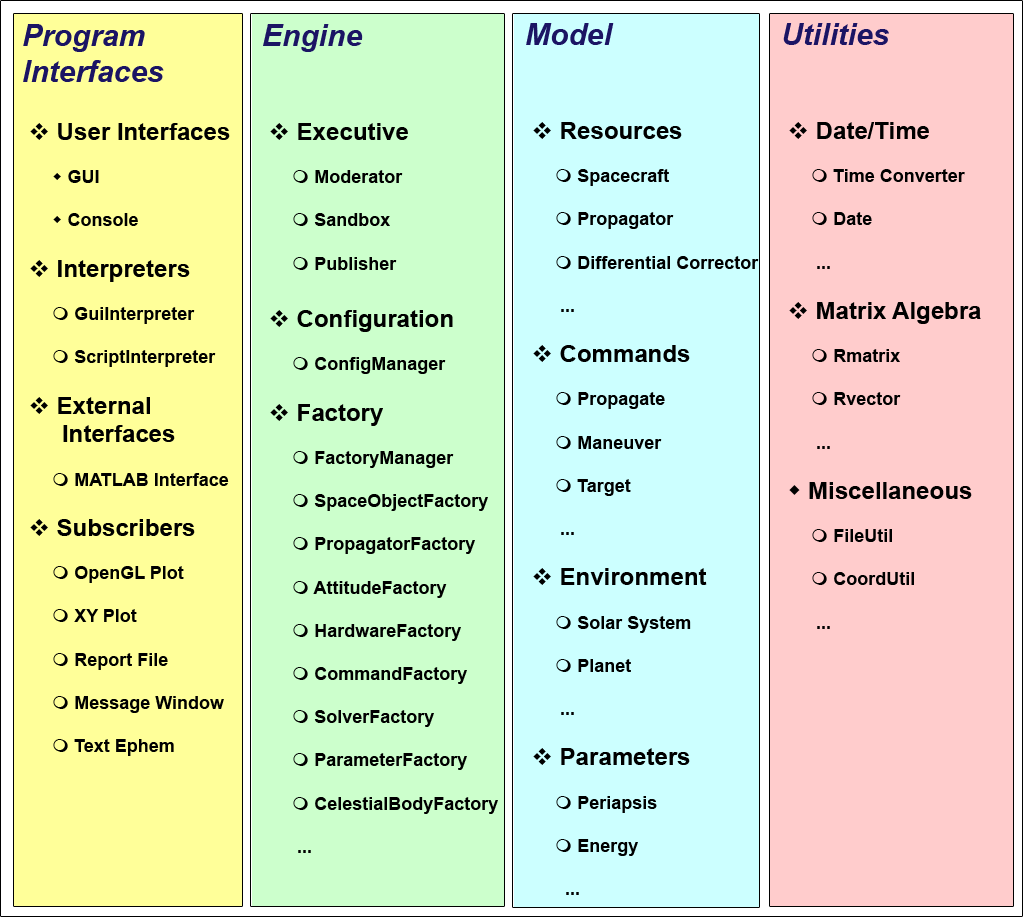
\includegraphics[scale=0.4]{Images/PackageHierarchy.eps}
\captionsetup{format=hang,justification=centerfirst,margin=96pt}
\caption[Packages, Subpackages, and Some Details]
{\label{figure:PackageHierarchy}Packages, Subpackages, and Some Details

Subpackages are indicated by a cluster of diamonds

Objects and Classes are marked by a circle

Other constructs are marked by a single diamond
}
\end{center}
\end{figure}

\begin{description}
\item[Program Interfaces] \index{Interfaces}All two-way communications between users and external
programs and GMAT are contained in the Program Interface package.  This package can be broken into
four subpackages:
  \begin{itemize}
    \item \textit{User Interfaces} \index{Interfaces!Program Interfaces}Users view GMAT through a
user interface -- usually through the GMAT Graphical User Interface (GUI), but also potentially
through a command line interface into GMAT called the GMAT console application, or Console.  These
interfaces are contained in the UserInterface subpackage.

    GMAT's GUI is coded using the wxWidgets cross-platform library\cite{wxWidgets}. The GUI provides
a rich environment that provides access to all of the features of GMAT through either panels
customized for each component or through a text based script.  Missions saved from the GUI are saved
in the script format, and scripts loaded into the GUI populate the GUI elements so that they can be
viewed on the customized interface panels.

    The console version of GMAT can be used to run script files and generate text data with little
user interaction.  The console application can run multiple scripts at once, or individual scripts
one at a time.  This version of the system is currently used for testing purposes, in situations
where the overhead of the full graphical user interface is not needed.

    \item \textit{Interpreters}\index{Interpreters!Overview} The user interface components
communicate with the core GMAT system through an interface layer known as the Interpreter
subpackage.  This layer acts as the connection point for both the scripting interface and the GUI
into GMAT.

    The Interpreter subpackage contains two specific interpreters: a GuiInterpreter, designed to
package messages between the GUI and the GMAT engine, and the ScriptInterpreter, designed to parse
script files into messages for the engine, and to serialize components in the engine into script
form for the purposes of saving these objects to file.

    The Interpreter subpackage is designed so that it can be extended to provide other means of
controlling the GMAT engine.  All that is required for this extension is the development of a new
interpreter, and interfaces for this new component into the Moderator, a component of the Executive
subpackage in GMAT's Engine package.

    \item \textit{External Interfaces} \index{Interfaces!External Interfaces}GMAT provides an
interface that can be used to communicate with external programs\footnote{At this writing, the only
external interface incorporated into the core GMAT code base is an interface to the MathWorks'
product MATLAB\cite{MATLAB}.}.  These interfaces are packaged in the ExternalInterfaces subpackage.

    \item \textit{Subscribers} \index{Interfaces!Subscribers}\index{Subscribers}Users view the
results of a mission run in GMAT through elements of the Subscriber subpackage.  Subscribers are
used to generate views of spacecraft trajectories, plots of mission parameters, and reports of
mission data in file form.

  \end{itemize}
  \item[The Engine] \index{Engine}The interfaces described above exist on top of a core simulation
engine used to control the model of flight dynamics problems in GMAT.  This engine consists of the
control and management structures for the program. The elements of the model used to simulate the
spacecraft mission are introduced in the next package description.  The Engine package consists of
three subpackages:
  \begin{itemize}
    \item \textit{Executive} \index{Engine!Executive Components}The Executive subpackage contains
the central processing component for GMAT (called the Moderator), a connection point used to capture
and distribute the results of a mission run (the Publisher), and the workspace used to run a mission
(the Sandbox).

    The Moderator acts as the central communications hub for the GMAT engine.  It receives messages
from the program interfaces through the interpreters, and determines the actions that need to be
taken based on these messages.  The Moderator sends messages to the other components of the Engine
to accomplish the requested tasks.

    GMAT is designed to run missions inside of a component called the Sandbox.  When a user requests
a mission run, the Moderator sets up the Sandbox with the elements configured for the run, and then
turns control over to the Sandbox to execute the mission.

    The Publisher acts as the connection between data generated in the Sandbox and the views of
these data presented to the User.  It receives data or instructional messages from the components in
the Sandbox, and passes those messages to the corresponding Subscribers.

    \item \textit{Configuration} \index{Engine!The Configuration}When GMAT builds a model, it starts
by building components that will be connected together based on a sequence of instructions.  Each
component is an instance of a GMAT class; as they are built, these components are stored in a local
repository of objects. The repository holding model components is known as the configuration.  The
Configuration subpackage consists of this repository and an interface used to access it, called the
ConfigurationManager.

    The components stored in the configuration are all derived from a base class named GmatBase,
described in Chapter~\ref{chapter:CoreClasses}.  In GMAT, every object that a user creates and uses
to simulate a spacecraft mission is derived from this base class.  The configuration is maintained
as a collection of pointers to GmatBase objects.  The ConfigurationManager works with this
collection to maintain the configuration repository.

    \item \textit{Factory} \index{Engine!Factories}\index{Factory!Overview}The model elements stored
in the configuration are created on request from the users.  The subpackage responsible for
processing requests for new model elements is the Factory subpackage.  It consists of an interface
into the subpackage -- the FactoryManager -- and a collection of factory classes used to create
specific types of model elements.

    Each factory in GMAT creates objects based on the type requested.  For example, Spacecraft or
Formation objects are created through a call is the corresponding type of object into the
SpaceObjectFactory.  Similarly, if a user needs a Prince-Dormand 7(8) integrator, a call is made to
the PropagatorFactory for that type of integrator.  The factory creates the object through a call to
the class's constructor, and returns the resulting object pointer.

    The Factory subpackage is constructed this way to facilitate extensibility.  Users can add user
generated classes by creating these classes and a Factory to instantiate them.  That factory can
then be registered with GMAT's FactoryManager, and users will be able to access their specialized
classes in GMAT without modifying the configured GMAT code base.  Eventually, users will be able to
load their objects through shared libraries (aka dlls in the Windows world) at run time.

    The FactoryManager registration process takes a factory and asks it what type of objects it can
create, and sends the corresponding requests to the correct factory.  Details of the factories
themselves can be found in Chapter~\ref{chapter:Factories}.  Extensibility is discussed in
Chapter~\ref{chapter:ExtendingGMAT}.
  \end{itemize}
  \item[The Model] \index{Model}The Engine package, described above, provides the programmatic
framework necessary for building and running a simulation in GMAT.  The objects that are used to
model the elements of the simulation are contained in the Model package.  All of the elements of the
Model package are derived from a common base class, GmatBase, described in
Chapter~\ref{chapter:CoreClasses}.

  When a user configures GMAT to simulate a spacecraft mission, the user is configuring objects in
the Model package.  In other words, the Model package contains all of the components that are
available to a user when setting up a mission in GMAT.  The model elements can be broken into four
subpackages:

  \begin{itemize}
    \item \textit{Environment} \index{Model!Environment}The environment subpackage provides all of
the background environmental data used in GMAT to model the solar system, along with the components
needed to perform conversions that require these elements.
    \item \textit{Resources} \index{Model!Resources}All of the model elements that do not require
some form of sequential ordering in GMAT are called Resources.  These are the model elements that
appear in the Resource tree in the GUI -- excluding the Solar System elements -- and they are the
elements that are stored in the configuration subpackage, described above.
    \item \textit{Commands} \index{Model!Commands}Commands are the elements of the model that
describe how the model should evolve over time.  Since commands are sequential, they are stored
separately, and in sequential order, in the Command subpackage.  The sequential set of commands in
GMAT is called the Mission Control Sequence.

    The Mission Control Sequence is a list of commands.  Commands that allow branching manage their
branches through ``child'' lists.  These branch commands can be nested as deep as is required to
meet the needs of the model.
    \item \textit{Parameters} \index{Model!Parameters}Parameters are values or data containers (e.g.
variables or arrays) that exist external to other objects in the GMAT model.  These objects are used
to perform calculations of data useful for analysis purposes.
  \end{itemize}
  \item[Utilities] \index{Utilities}The Utility package contains classes that are useful for
implementing higher level GMAT functions.  These core classes provide basic array computations, core
solar system independent calculations, and other useful low level computations that facilitate
programming in the GMAT system.
\end{description}

\subsection{Package Component Interactions}

The preceding section provides a static view into the components of GMAT.  In this section, a
high level view of the interactions between the elements of these packages will be described.
Figure~\ref{figure:TopLevelPackages} shows the static package view of GMAT.  Each top level package
is color coded so that the system components shown in the interaction diagram,
Figure~\ref{figure:GMATStackDiagram}, can be identified with their containing package.  The legend
on this figure identifies the package color scheme.

\begin{figure}
\begin{center}
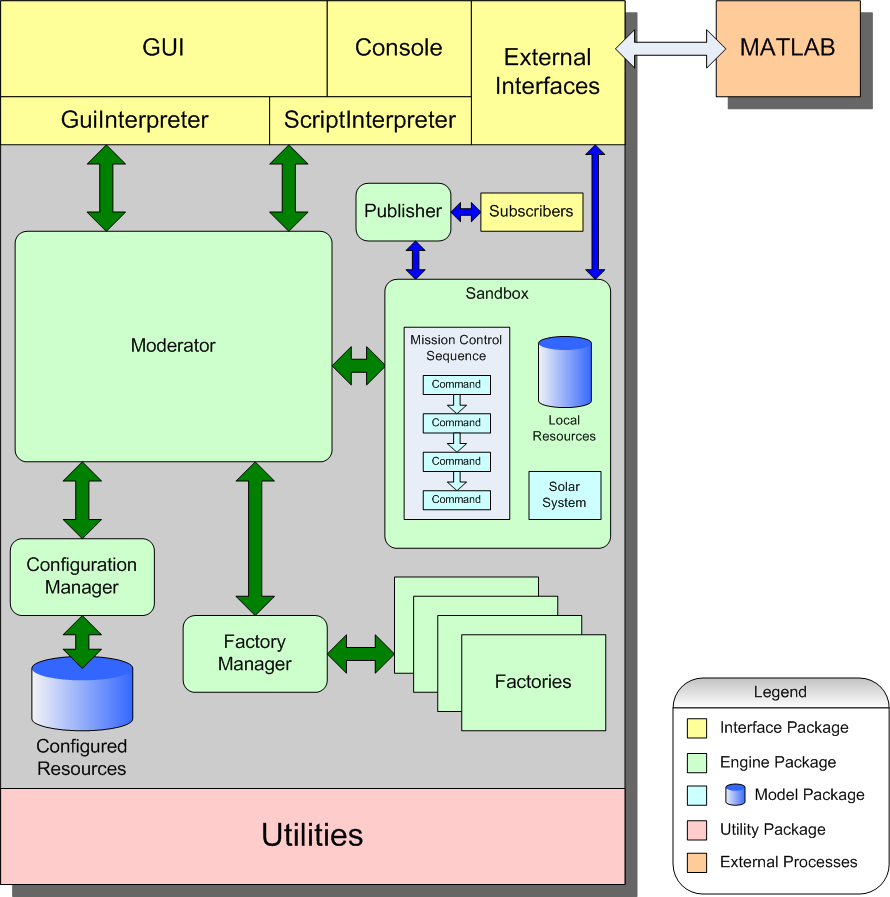
\includegraphics[scale=0.5]{Images/GMAT_Stack.eps}
\caption[Subsystem Interactions in GMAT]{\label{figure:GMATStackDiagram}Subsystem Interactions in
GMAT\\Green arrows show information flow between the core Engine components, while blue arrows show
information flow that occurs when a mission is executed.}
\end{center}
\end{figure}

Users interact with GMAT through either a Graphical User Interface (GUI) written using the
cross-platform GUI library wxWidgets, or through a console-based application designed to
run scripts without displaying graphical output.  These interfaces communicate with the GMAT engine
through interpreter singletons\footnote{\index{Singleton}\index{Design Patterns!Singleton}The GMAT
engine is run through a set of singleton class instances.  The singleton design pattern used for
these instances is introduced in Appendix~\ref{chapter:Patterns}.  The important thing to know about
singletons for this discussion is that there is only one instance of any singleton class; hence a
running GMAT executable has one and only one ScriptInterpreter, and Moderator, and at most one
GUIInterpreter.  Other singletons will be introduced during this discussion as well, when the
factories and configuration are discussed.}.  The GUI application interacts with the engine through
both the Script and GUI Interpreters, while the console application interacts through the script
interpreter exclusively.  These interpreters are designed to mediate two-way communications between
the GMAT engine and users.   The GUI and console applications drive the GMAT engine through these
interpreters.

The Interpreters in turn communicate with GMAT's Moderator singleton.  The Moderator is the central
control object in the GMAT engine.  It manages all program level communications and information flow
while the program is running.  It receives messages from the interpreters, processes those messages,
and instructs other components of the engine to take actions in response to the messages.  The
messages sent by the interpreters fall into several distinct groups:

\begin{itemize}
\item\textbf{Object Creation} messages are used to request the creation of resources stored in the
configuration database or the creation of commands stored in the Mission Control Sequence.
\item\textbf{Object Retrieval} messages are used to access created objects, so they can be modified
by users or stored to file.
\item\textbf{Run} messages prepare the Sandbox for a run of the Mission Control Sequence, and then
launch execution of the Mission Control Sequence.
\item\textbf{Polling} messages are used to control an executing Mission Control Sequence, and are
used to coordinate external communications (for example, the startup process for MATLAB) and user
actions taken during the run.
%\item\textbf{Reset} messages are used to clear the configuration database and Mission Control
% Sequence so that a new model can be built in the engine.
\end{itemize}

\noindent The message and information flow in the Engine are shown in
Figure~\ref{figure:GMATStackDiagram} with double headed arrows.  The green arrows show the central
message and information flow in the engine, while the blue arrows show information flow that occurs
while a mission control sequence is executing.  These messages are described briefly here, and more
completely through examples later in this chapter.

The Moderator responds to requests for new resources or commands by requesting a new object from the
FactoryManager.  The FactoryManager determines which Factory class can supply the requested object,
and sends a ``create'' request to that factory.  The Factory builds the requested object, and sends
the pointer to the new object to the FactoryManager, which in turn sends the pointer to the
Moderator.  The Moderator sends the new object's pointer to one of two locations, depending on the
type of object created.  If the object is a Resource, the object pointer is passed to the
ConfigurationManager.  The ConfigurationManager adds the resource to the database of configured
objects.  If the requested object is a command, it is added to the Mission Control Sequence.  The
Moderator then returns the pointer to the interpreter that requested the new object.

Object retrieval is used to retrieve the pointer to an object that was previously created.  The
Moderator receives the message asking for the object.  If the object is a configured resource, it
calls the ConfigurationManager and asks for the resource by name.  Otherwise, it traverses the
Mission Control Sequence until it finds the requested command, and returns the pointer to that
command.

% Trying to fix a small nit with figure placement here
\begin{figure}
\begin{center}
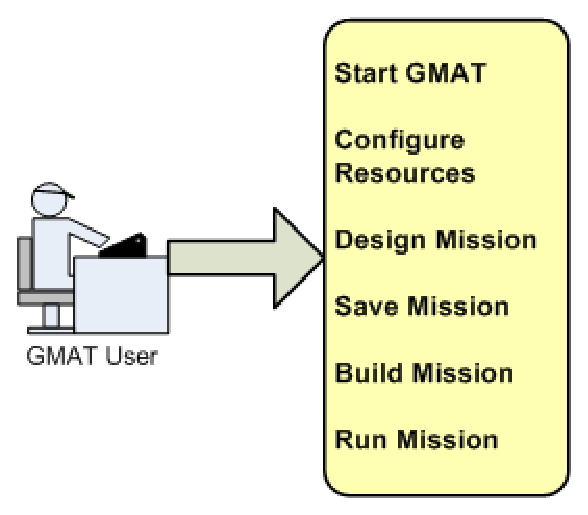
\includegraphics[scale=0.5]{Images/GMAT_UserPerspective.eps}
\caption{\label{figure:UserWorkFlow}User Interactions}
\end{center}
\end{figure}

Run messages are used to transfer the resources and Mission Control Sequence into the Sandbox and
start a run of the mission.  When the Moderator is instructed to run a Mission Control Sequence, it
starts by loading the configured components into the Sandbox.  The Moderator requests objects from
the ConfigurationManager, by type, and passes those objects to the Sandbox.  The Sandbox receives
the object pointers, and clones each object into a local resource database.  These local clones are
the objects that interact with the commands in the Mission Control Sequence to run a mission.  The
Moderator then passes the Mission Control Sequence to the Sandbox so that the Sandbox has the list
of commands that need to be executed to run the mission.  Next Moderator tells the Sandbox to
initialize its components.  The Sandbox initializes each of the local components, and establishes
any necessary connections between components in response to this message.  Finally, the Moderator
instructs the Sandbox to execute the Mission Control Sequence.  The Sandbox starts with the first
command in the sequence, and runs the commands, in order, until the last command has executed or the
run is terminated by either a user generated interrupt or an error encountered during the run.

Polling messages are used to process messages between the Moderator and the Sandbox during a run.
Typical messages processed during polling are user requests to pause or terminate the run, or to
open a connection to an external process (including the startup of that process).

The descriptions provided here for these message types may be a bit confusing at first.  The
following section provides representative cases of the message passing and object interactions in
GMAT when a user performs several common interactions.

\section{\label{section:TopLevelUseCase}GMAT Workflow Overview}

When users run GMAT, they follow a work flow like that shown in Figure~\ref{figure:UserWorkFlow}.
Users start the program, configure resources, plan their mission, save the configuration, build the
mission if working from a script file, and run the mission.  The following sections describe the top
level actions taken by GMAT when a user initiates each of these actions.

\subsection{\label{section:GMATStartup}The GMAT Startup Process}\index{Startup}

\begin{figure}[htb]
\begin{center}
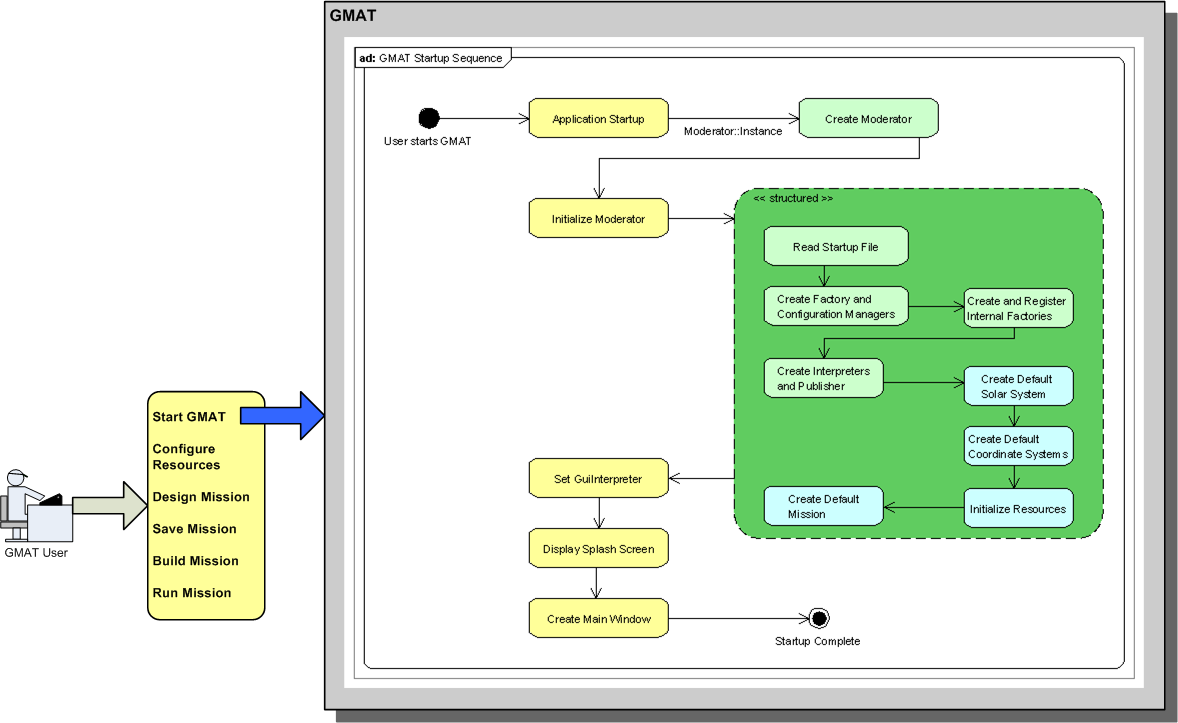
\includegraphics[scale=0.35]{Images/GMAT_Startup.eps}
\caption{\label{figure:StartupActivities}The Startup Process}
\end{center}
\end{figure}

The startup process for GMAT, shown in Figure~\ref{figure:StartupActivities}, launches the
executable program and prepares the engine for use.  Most of the work performed during startup is
performed by the Moderator.  When the application launches, the first action taken is the creation
of the Moderator singleton, made by calling the static Instance() method on the Moderator class.
This freshly created Moderator is then initialized by the application through a call to the
Initialize{} method.

The procedure followed in Initialize() is shown in the large green structured flow box in the
figure.  The Moderator reads the GMAT startup file, setting linkages to the default files needed to
model and display running missions.  The startup file resides in the same folder as the GMAT
application, and contains path and file information for planetary ephemerides, potential models,
graphical images used to provide texture maps for bodies displayed in the GUI, atmospheric model
files, and default output paths for log files and other GMAT generated outputs.

Upon successful read of the startup file, the Moderator starts creating and connecting the main
components of the engine.  It begins by creating the components used for building model elements.
The FactoryManager and ConfigurationManager are created first.  Next the Moderator creates each of
the internally configured factories, one at a time, and passes these instances into the
FactoryManager.  This process is called ``registering'' the Factories in other parts of this
document.  Upon completion of Factory registration, the Moderator creates instances of the
ScriptInterpreter and GuiInterpreter singletons and the Publisher singleton.  This completes the
configuration of the core engine elements, but does not complete the Moderator initialization
process, because GMAT starts with several default model elements.

The Moderator creates a default Solar System model, populated with a standard set of solar system
members.  Next it creates three default coordinate systems that always exist in GMAT configurations:
the Earth-Centered Mean of J2000 Earth Equator system, the Earth-Centered Mean of J2000 Ecliptic
system, and the Earth-Centered Earth body-fixed system.  Next the Moderator sets the pointers
needed to interconnect these default resources.  Finally, the Moderator creates a default mission,
and upon success, returns control to the GMAT application.

The Application retrieves the pointer for the GuiInterpreter, and sets this pointer for later use in
the GUI.  It then displays the GMAT splash screen, and then finally creates and displays the main
GMAT Window.  At this point, the GMAT GUI is configured and ready for use building models and
running missions.

\subsection{Configuring Resources}\index{Model!Resources}

\begin{figure}[htb]
\begin{center}
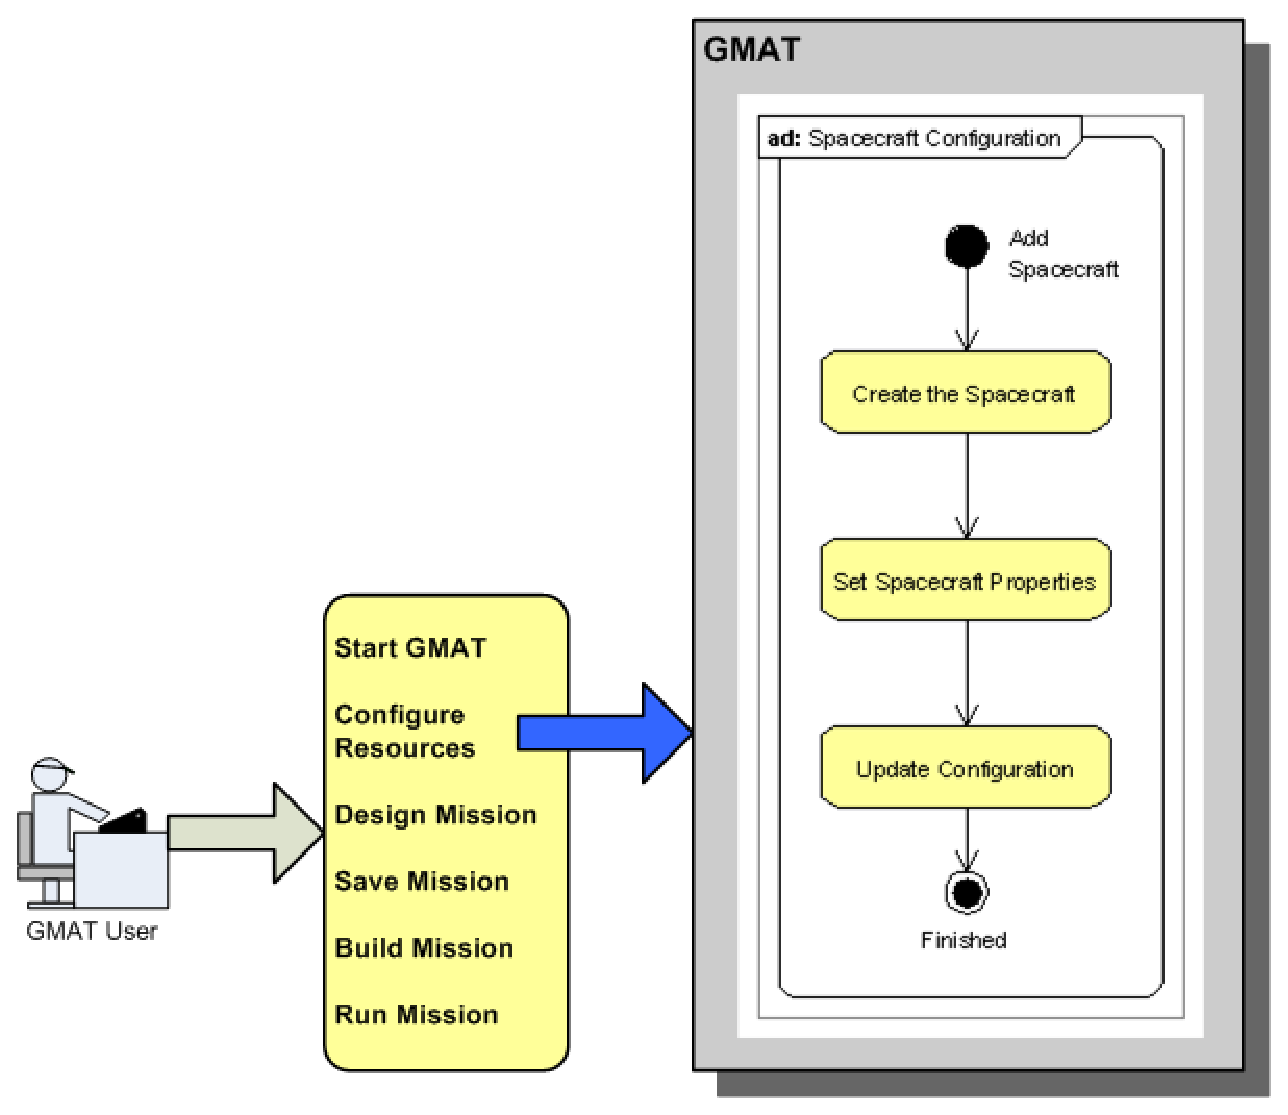
\includegraphics[scale=0.4]{Images/GMAT_ConfigureResource.eps}
\caption{\label{figure:ResourceConfig}Configuration Example: Spacecraft}
\end{center}
\end{figure}

Figure~\ref{figure:ResourceConfig} shows the top level set of actions taken by a user when
configuring a typical resource -- in this case, a Spacecraft object -- from the GUI.  The user
starts by using a right click on the Spacecraft folder (or control-click on the Mac) in the
resource tree on the left side of the main GMAT window.  This action opens a context menu; the user
selects ``Add Spacecraft'' from this menu, and a new spacecraft resource appears in the resource
tree.  This action is represented by the box labeled ``Create the Spacecraft'' in the figure.  The
user may also elect to change the name of the new Spacecraft.  This action is taken with a right
click (control-click on the Mac) on the new resource in the resource tree, and selecting
``Rename'' from the resulting context menu.

Once a resource has been created, the user can edit the properties of the resource.  From the GUI,
this action is performed with a double click on the resource.  The double click opens a new panel
tailored to the type of resource that is selected; for a Spacecraft, the panel shown in
Figure~\ref{figure:SpacecraftConfigPanel} opens.  The second block in
Figure~\ref{figure:ResourceConfig}, labeled ``Set Spacecraft Properties'', represents the actions
taken in GMAT when the user performs this selection, and when the user makes changes on the
resulting panel.

\begin{figure}[htb]
\begin{center}
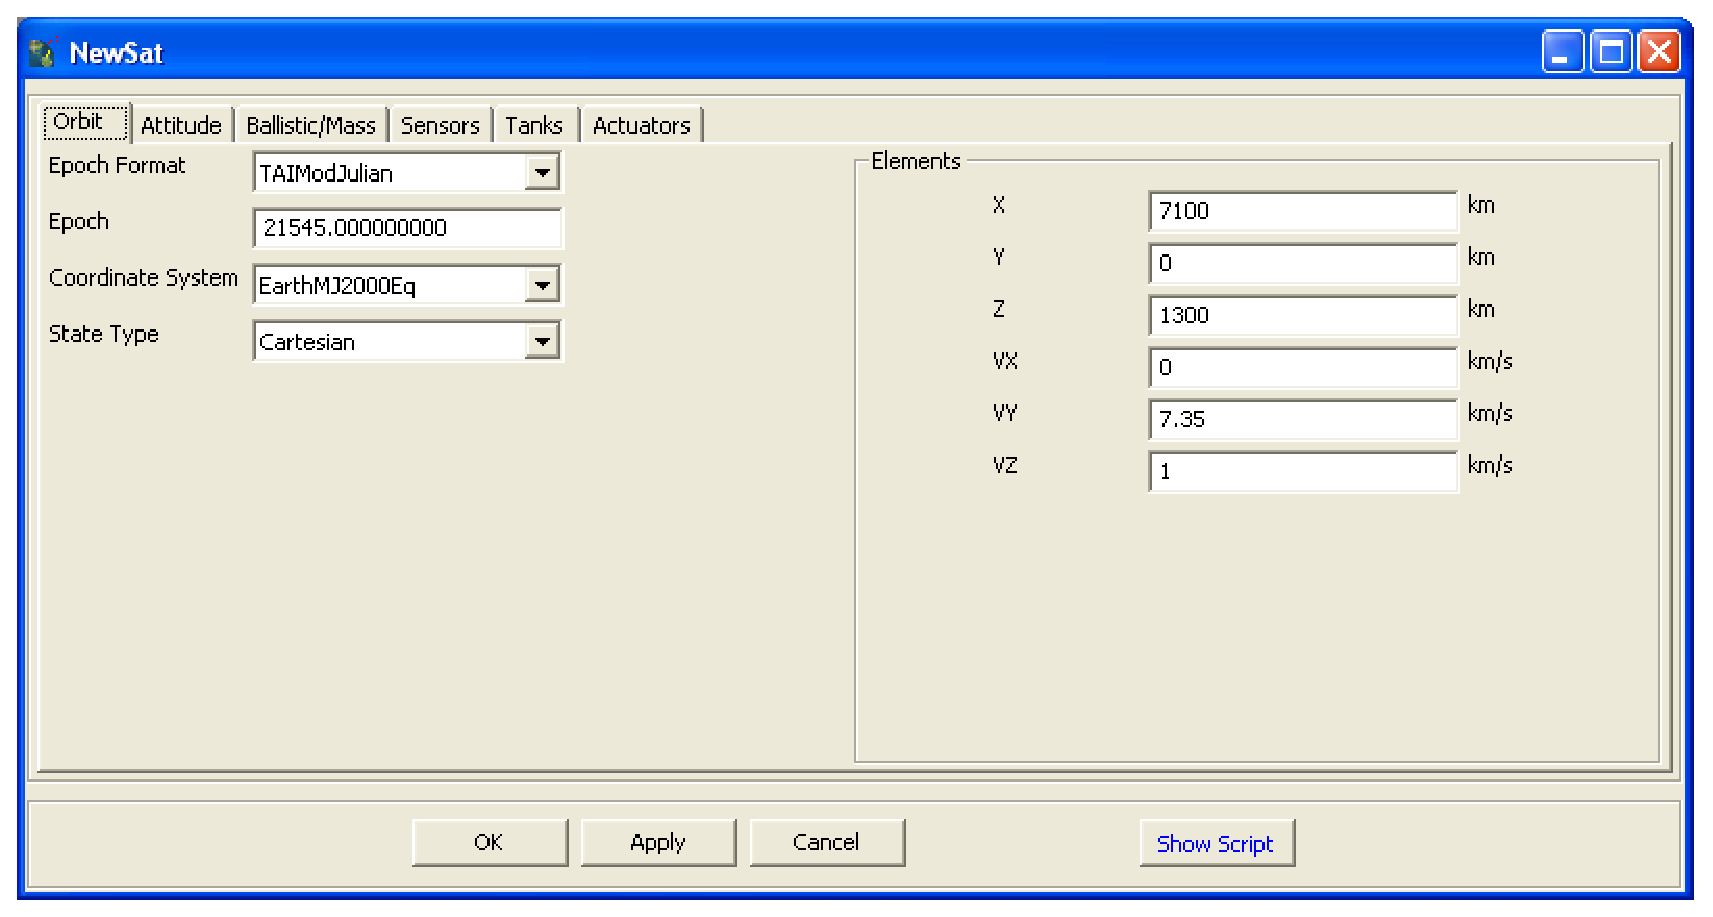
\includegraphics[scale=0.5]{Images/SpacecraftPanel.eps}
\caption{\label{figure:SpacecraftConfigPanel}The Spacecraft Configuration Panel}
\end{center}
\end{figure}

Changes made in a GUI panel like the one shown here are not automatically made on the underlying
objects in GMAT.  Changes made on the panel are fed back to the internal objects when the user
selects either the ``Ok'' or ``Apply'' button on the bottom of the panel.  This updating of the
resource is represented by the ``Update Configuration'' block in Figure~\ref{figure:ResourceConfig}.

Each of these blocks can be further decomposed into the internal actions performed in GMAT when the
user makes the selections described here.  The following paragraphs describe in some detail how GMAT
reacts to each of these user actions.

\subsubsection{\label{section:ObjectCreation}Creating the Spacecraft}

\begin{figure}[htb]
\begin{center}
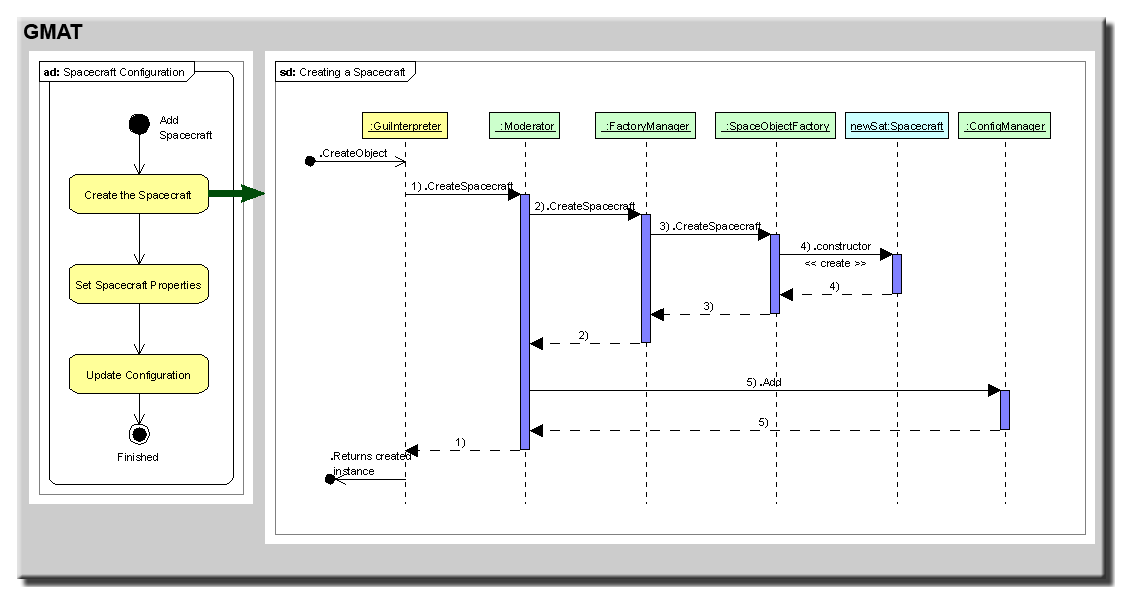
\includegraphics[scale=0.8]{Images/SpacecraftCreation.eps}
\caption[Configuration Example: Creating the
Spacecraft]{\label{figure:CreatingResource}Configuration Example: Creating the Spacecraft}
\end{center}
\end{figure}

Figure~\ref{figure:CreatingResource} shows an example of the process followed in GMAT when a new
resource is created from the GUI.  The user selected ``Add Spacecraft'' from the option menu on the
Spacecraft node of the resource tree (accessed with a right click -- control-click on the Mac -- on
the node).  This selection triggered the chain of events shown in the sequence diagram in the
figure\footnote{For an introduction to the UML diagram notation used throughout this document, see
Appendix~\ref{chapter:UMLDiagrams}}.  The sequence starts with a CreateObject() call from the GUI to
the interface into the GMAT engine.  The interface between the GUI and the GMAT engine is a
singleton instance\footnote{Singletons, and other design patterns used in GMAT, are introduced on
Appendix~\ref{chapter:Patterns}.} of the GuiInterpreter class, and is shown in green in the figure.

The GuiInterpreter singleton receives the call to create an object of type Spacecraft.  It makes a
call, in turn, into the singleton responsible for running the GMAT engine.  This singleton is an
instance of the Moderator class\footnote{For the purposes of this discussion, the singleton
instances will be referred to by their class name for the remainder of this discussion.}.  The call
into the Moderator is made in step 1 of the diagram; the call is made through the CreateSpacecraft()
method of the Moderator.

User configured objects in GMAT are always created through calls into a subsystem referred to
collectively as the Factory subsystem.  Factories are responsible for creating these objects.  The
factory subsystem is managed through a singleton class, the FactoryManager.  The Moderator accesses
the factories through this singleton.  In step 2 of the figure, the Moderator makes a call to the
CreateSpacecraft() method on the FactoryManager.  The FactoryManager finds the Factory responsible
for creating objects of the type requested -- in this case, a Spacecraft object -- and calls that
factory in turn.  Spacecraft are created in GMAT's SpaceObjectFactory, so the FactoryManager calls
the CreateSpacecraft() method on the SpaceObjectFactory, as is shown in step 3.

The SpaceObjectFactory creates an instance of the Spacecraft class by calling the class's
constructor, as shown in step 4.  The constructed object is given a name, and then returned
through the FactoryManager to the Moderator.  The Moderator receives the new object, and adds it to
the database of configured objects in GMAT.

All configured GMAT objects are managed by a singleton instance of the ConfigurationManager class.
The ConfigurationManager is used to store and retrieve objects during configuration of the model.
The Moderator adds created components to the configuration by calling Add() methods on the
ConfigurationManager.  For this example, the new Spacecraft is added to the configuration through
the call shown in step 5.

Once the steps described above have been completed successfully, the Moderator returns control to
the GuiInterpreter, which in turn informs the GUI that a new object, of type Spacecraft, has been
configured.  The GUI adds this object to the resource tree, and returns to an idle state, awaiting
new instructions from the user.

\subsubsection{\label{section:ObjectConfiguration}Setting Spacecraft Properties}

The Spacecraft that was created above has default settings for all of its properties.  Users will
typically reset these properties to match the needs of their mission.  The process followed for
making these changes from the GUI is shown in Figure~\ref{figure:ConfiguringResource}.

\begin{figure}[htb]
\begin{center}
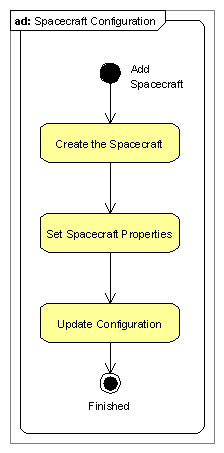
\includegraphics[scale=0.35]{Images/SpacecraftConfiguration.eps}
\caption{\label{figure:ConfiguringResource}Configuration Example: Setting Spacecraft Properties}
\end{center}
\end{figure}

As was discussed in the introduction to this section, Spacecraft properties are set on the GUI panel
shown in Figure~\ref{figure:SpacecraftConfigPanel}.  Users can open this panel at any point in the
model setup process.  Because of the free flow in the configuration process, the Spacecraft pointer
may not be accessible when the user elects to open the configuration panel with a double click on
the Spacecraft's name on GMAT's resource tree.  Therefore, the first action taken when the panel is
opened is a call from the panel to the GuiInterpreter to retrieve the configured Spacecraft with the
name as specified on the Resource tree.  The GuiInterpreter passes this request to the Moderator.
The Moderator, in turn, asks the ConfigurationManager for the object with the specified name.  The
ConfigurationManager returns that object to the Moderator, which passes it to the GuiInterpreter.
The GuiInterpreter returns the object (by pointer) to the Spacecraft Panel.

The Spacecraft Panel creates a temporary clone of the configured spacecraft so that it has an object
that can be used for intermediate property manipulations\footnote{The Spacecraft is unique in this
respect; other objects configured in the GMAT GUI are manipulated directly, rather than through a
clone.  The Spacecraft is in many respects a composite object; this added complexity makes the
intermediate clone a useful construct.}.  This clone is set on the Spacecraft Panel's subpanels,
accessed through a tabbed interface shown in the snapshot of the panel.  Each subpanel accesses the
properties corresponding to the fields on the subpanel, and sets its data accordingly. The
Spacecraft Panel is then displayed to the user.  The user then makes any changes wanted for the
model that is being configured.

\subsubsection{\label{section:ObjectPersistance}Saving the Spacecraft}

\begin{figure}[htb]
\begin{center}
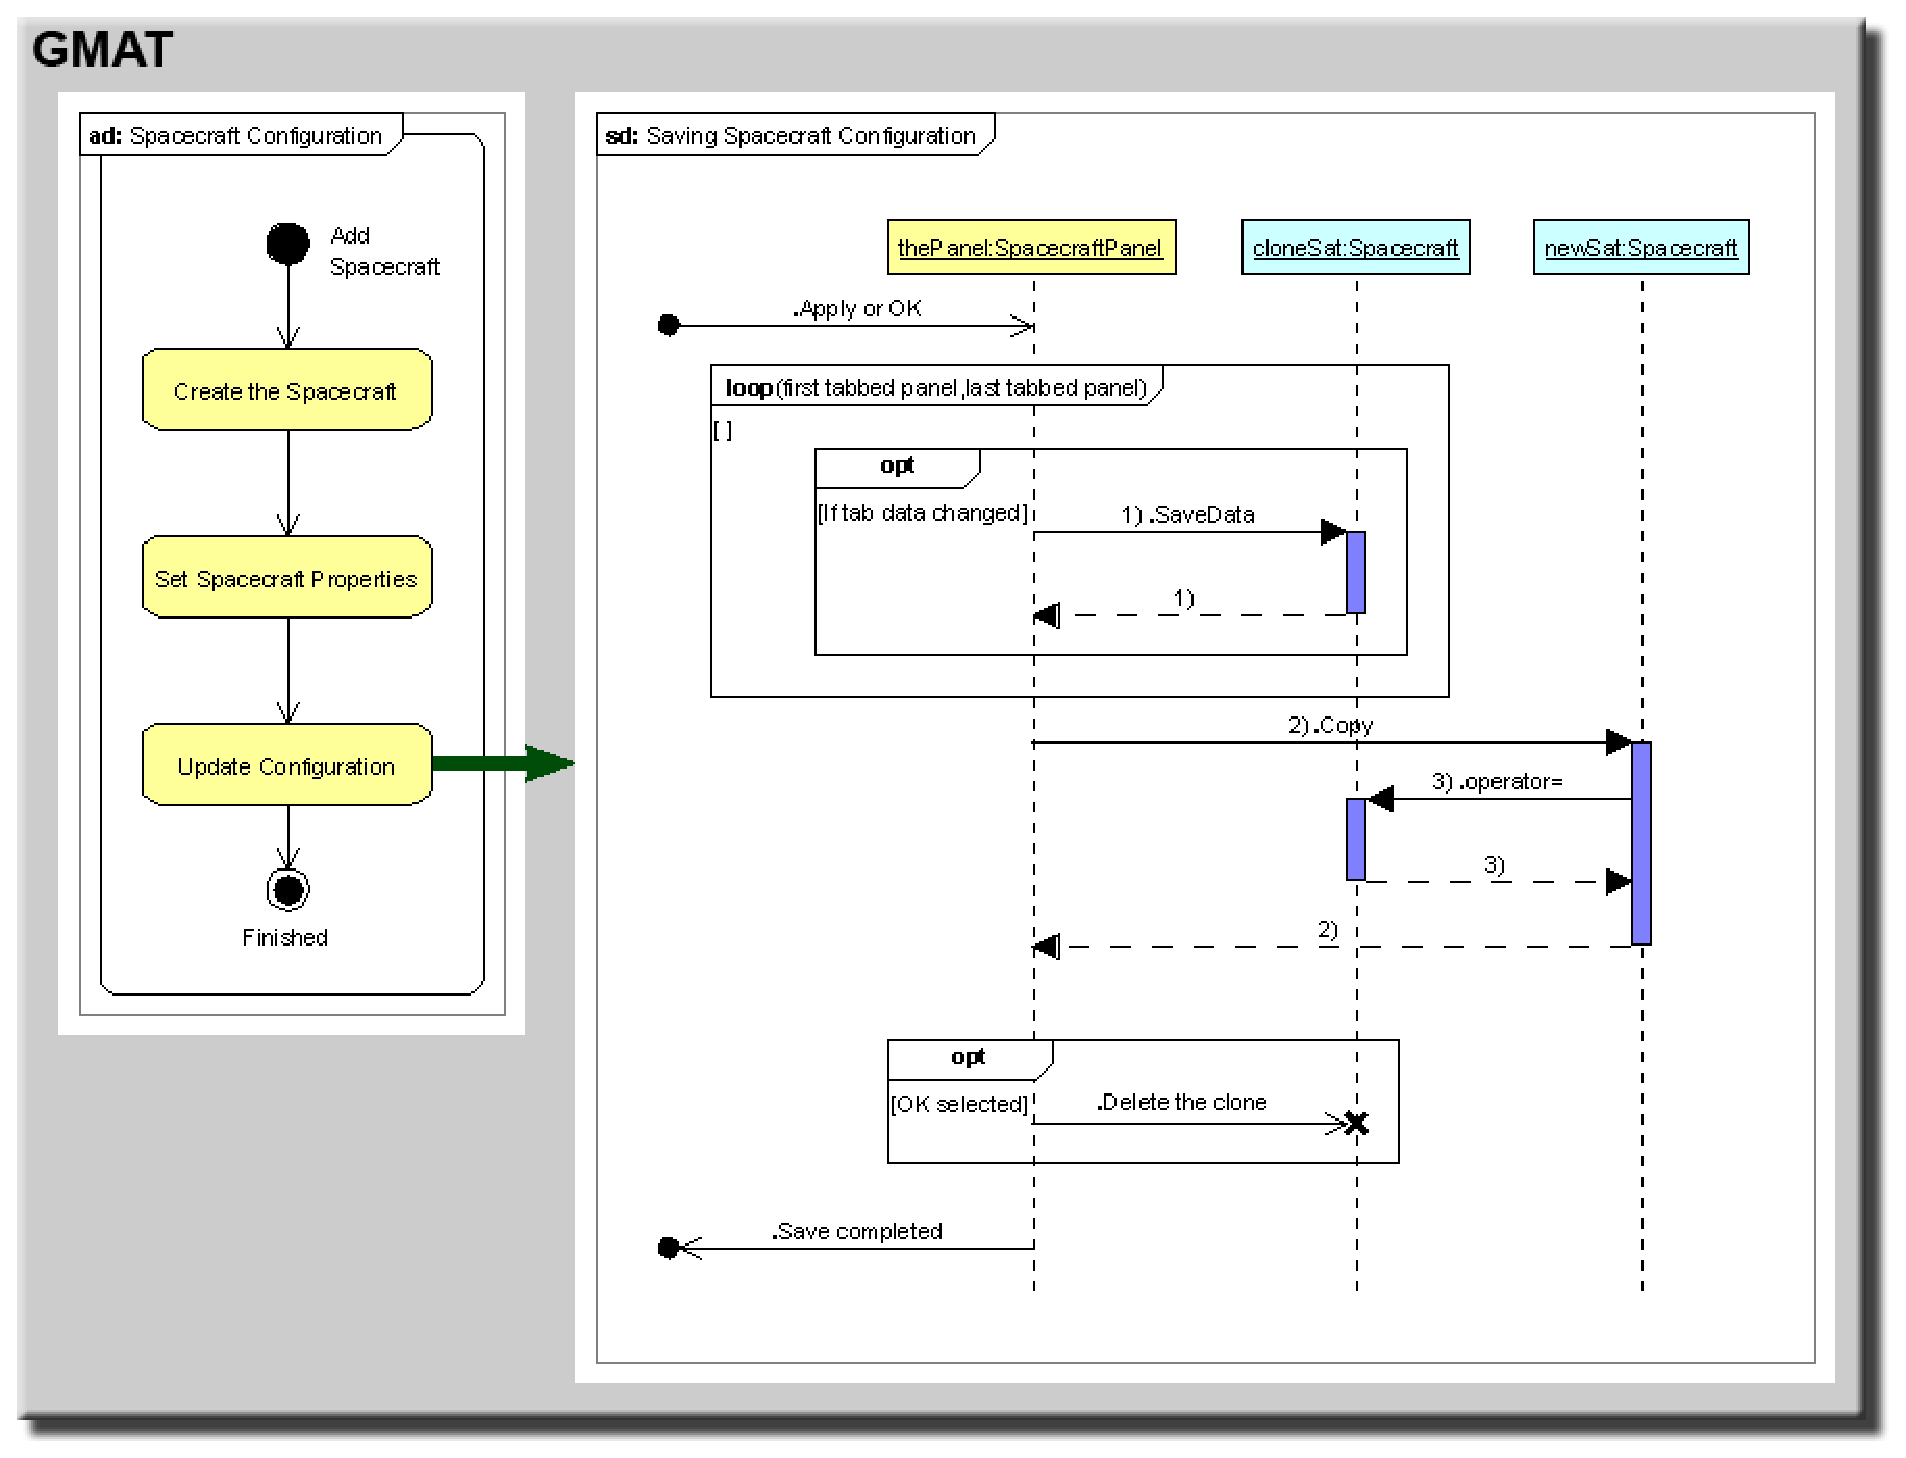
\includegraphics[scale=0.5]{Images/SpacecraftSave.eps}
\caption{\label{figure:SavingResource}Configuration Example: Saving the Spacecraft}
\end{center}
\end{figure}

The final step in the spacecraft configuration process is saving the updated data into the
configuration.  That process is shown in Figure~\ref{figure:SavingResource}.

The Spacecraft Panel has several tabbed subpanels.  The SpacecraftPanel begins the save process by
calling each of these subpanels in turn, setting the corresponding Spacecraft data one subpanel at a
time on the locally cloned Spacecraft.  Once all of the subpanels have synchronized their data with
the clone, the copy constructor of the configured Spacecraft is called with the cloned Spacecraft as
the input argument.  This action updates the configured Spacecraft, completing the save action.

There are two buttons on the Spacecraft Panel that can be used to perform the save action.  The
button labeled ``Apply'' saves the updated data to the configured object and leaves the Spacecraft
Panel open for further user manipulation.  The ``OK'' button saves the data and closes the panel.
The latter action destroys the instance of the panel.  Since the panel is going out of scope, the
cloned Spacecraft must also be deleted, as is shown in the figure.

\subsection{Configuring Commands}\index{Model!Commands}

The previous paragraphs describe the interactions between core GMAT components and the internal
message passing that occurs when a component of a GMAT Model is configured for use.  The following
paragraphs describe the analogous configuration for the commands in the Mission Control Sequence.

\begin{figure}[htb]
\begin{center}
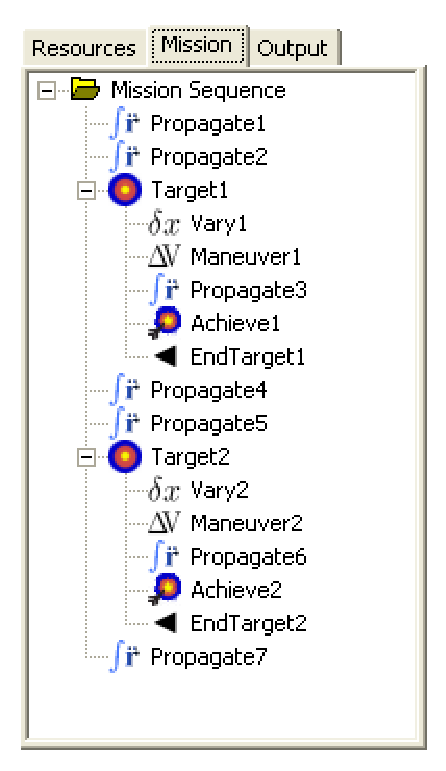
\includegraphics[scale=0.5]{Images/MissionTree.eps}
\caption{\label{figure:MissionTree}The Mission Tree in GMAT's GUI}
\end{center}
\end{figure}

The Mission Control Sequence is shown in the GMAT GUI on the tab labeled ``Mission,'' shown for a
modified Hohmann transfer problem\footnote{The modification made here is along the transfer
trajectory from the initial orbit to the final orbit.  The spacecraft in this example is propagated
through one and a half orbits on the transfer trajectory, rather than the typical half orbit needed
for the problem.} in Figure~\ref{figure:MissionTree}.  The sequence is shown as a hierarchical tree
of commands.  Each level of the hierarchy is a separate list of commands.  The top level list is the
main control sequence.  Commands that branch from this list are shown indented one level from this
sequence.  Commands branching off of these commands are indented an additional level\footnote{In
some cases sequences of similar commands are also indented to simplify the display of the Mission
Control Sequence.}.  This process continues until all of the commands in the sequence are
incorporated into the tree structure.

The Mission Control Sequence shown in the figure consists of seventeen commands, grouped as seven
commands in the main (i.e. top level) sequence, five additional commands branched off of this
sequence to perform one set of maneuver targeting, and an additional five commands to perform
targeting for a second maneuver.  The main sequence of commands shown here is the sequence Propagate
-- Propagate -- Target -- Propagate -- Propagate -- Target -- Propagate.  The Target commands are
used to tune the maneuvers at each end of the transfer orbit by applying the command sequence Vary
-- Maneuver -- Propagate -- Achieve -- EndTarget.  The inner workings of these commands is beyond
the scope of this chapter; the important thing to observe at this point is the sequencing of the
commands, and the presentation of this sequencing to the user by way of GMAT's GUI.

The tree shown in the GUI is populated by traversing the linked list of commands comprising the
Mission Control Sequence.  Each node of the Mission Tree is an instance of the class
MissionTreeItemData.  This class includes a pointer to the corresponding GmatCommand object in the
Mission Control Sequence.  When GMAT needs to build or refresh the Mission Tree, it accesses the
first node in the Mission Control Sequence and creates a corresponding MissionTreeItemData instance.
That instance is passed the pointer to the GmatCommand, and uses that command pointer to configure
its properties in the tree.  GMAT then asks for the next node in the sequence, and repeats this
operation until the tree is fully populated.

Some GmatCommands are derived from a subclass named BranchCommand.  These commands manage child
linked lists, like the ones shown for the target commands in the figure.  When the GUI encounters a
BranchCommand derivative, it indents the nodes displayed on the Mission Tree to indicate this nested
level for the child sequence of the branch command.  All of the commands that allow this type of
nesting are terminated with a corresponding ``End'' command -- for this example, the Target command
terminates the targeting child sequence when it encounters an EndTarget command.

Users interact with the Mission Control Sequence either through GMAT's scripting interface, or
through manipulations made in the GUI.  Manipulations made while scripting are pretty
straightforward; they consist of editing a script file of commands and then instructing GMAT to
parse this script.  This process will be described later.  Figure~\ref{figure:CommandConfig} shows
the steps a user takes when adding a command to the Mission Control Sequence from the GUI.

\begin{figure}[H]
\begin{center}
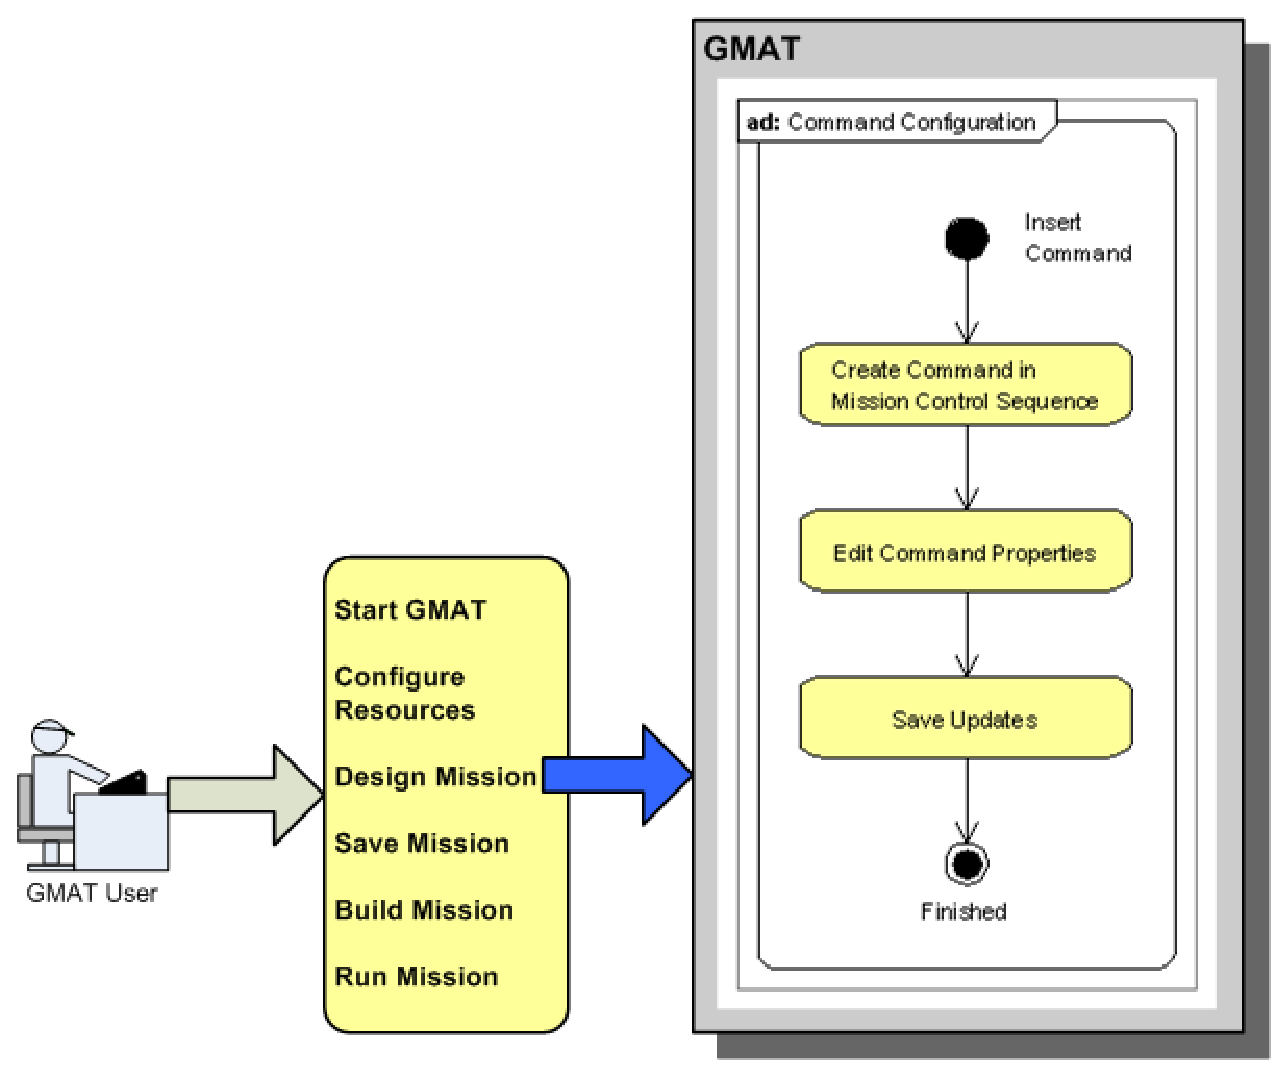
\includegraphics[scale=0.5]{Images/GMAT_ConfigureCommand.eps}
\caption{\label{figure:CommandConfig}Configuration Example: A Mission Control Sequence Command}
\end{center}
\end{figure}

The Mission Control Sequence is a doubly linked list of objects that describes the sequence of
actions that GMAT will run when executing a mission.  Each node in the linked list is an object
derived from the command base class, GmatCommand, as is described in Chapter~\ref{chapter:Commands}.
 Since GmatCommand objects are doubly linked in the list, each command has a pointer to its
predecessor and to the next command in the list.  When a user decides to add a command to the
Mission Control Sequence, a node in the Mission tree is selected and right clicked (or
control-clicked on the Macintosh).  This action opens a context menu with ``Insert Before'' and
``Insert After'' submenus as options.  The ``Before'' and ``After'' selections here refer to the
location of the new command.  The user selects the desired command type from the submenu, and the
requested command is added to the Mission Control Sequence in the specified location.  This set of
actions corresponds to the first block in the activity diagram, labeled ``Create Command in Mission
Control Sequence.''

Most of the commands in GMAT require additional settings to operate as the user intends -- for
example, Propagate commands require the identity of the propagator and spacecraft that should be
used during propagation.  The second block in the figure, ``Edit Command Properties,'' is launched
when the user double clicks on a command.  This action opens a command configuration panel designed
to help the user configure the selected command.  The user edits the command's properties, and then
saves the updates back to the command object by pressing either the ``Apply'' or ``OK'' button on
the panel.  This action is performed in the ``Save Updates'' block in the figure, and is the final
step a user takes when configuring a command.

Each of these high level actions can be broken into a sequence of steps performed between the core
elements of GMAT, as is described in the following paragraphs, which describe the interactions
followed to add a Maneuver command to the Mission Control Sequence.

\subsubsection{\label{section:CommandCreation}Creating a Maneuver Command}

Figure~\ref{figure:ManeuverCreation} shows the process followed when a Maneuver command is created
and inserted following an existing command from the GMAT GUI.  The process starts when the user
selects a command on the mission tree, right clicks it, and chooses the ``Insert After'' option
from the resulting context menu.  The resulting submenu contains a list of available commands; the
following actions occur when the user selects ``Maneuver'' from this list.

\begin{landscape}
\begin{figure}[htb]
\begin{center}
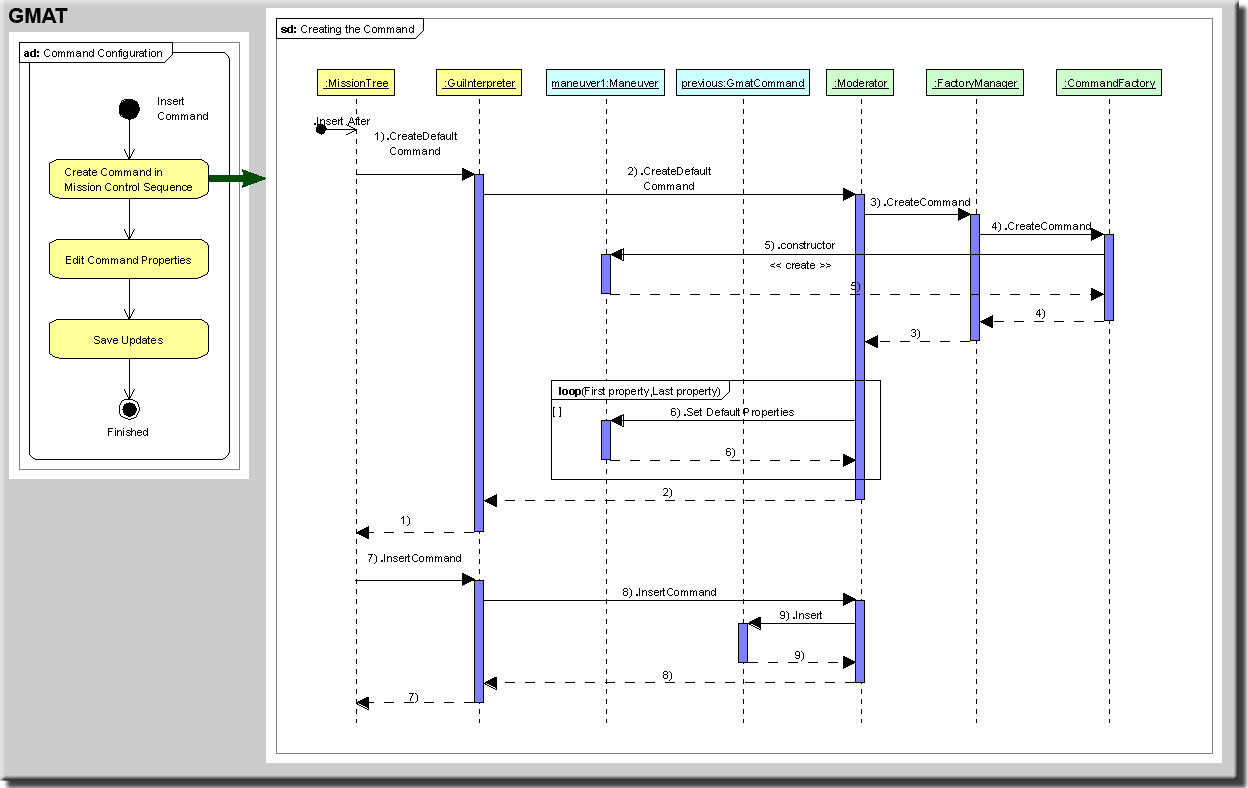
\includegraphics[scale=0.9]{Images/ManeuverCreation.eps}
\caption{\label{figure:ManeuverCreation}Command Creation Example: Creating a Maneuver Command}
\end{center}
\end{figure}
\end{landscape}

Maneuver command creation starts when the MissionTree\footnote{Here, and throughout this document,
specific instances of singleton classes are referred to by the class name -- ``MissionTree'' in this
case.  When the class or user experience of the instance is discussed, it will be referred to
 less formally -- ``mission tree'', for example.  So as an example of this style, we might discuss
the user selecting an object on the mission tree in the GUI, which causes the MissionTree to perform
some action.} object sends a request to the GuiInterpreter for a new Maneuver command instance. The
GuiInterpreter sends the request to the Moderator, which sends the request to the FactoryManager.
The FactoryManager finds the factory that creates Maneuver commands, and asks that factory for an
instance of the Maneuver command.  The resulting instance is returned from the factory, through the
FactoryManager, to the Moderator.  The Moderator sets some default data on the command, and then
returns the command pointer to the GuiInterpreter. The GuiInterpreter passes the command pointer to
the MissionTree.

Each node in the MissionTree includes a data member pointing to the corresponding command in the
Mission Control Sequence.  This structure simplifies the interactions between the GUI and the engine
when a user makes changes to the Mission Control Sequence.  Since the MissionTree already has a
pointer to the command preceding the new Maneuver command, it has all of the information needed to
request that the new command be added to the Mission Control Sequence.  The new Maneuver command is
added to the Mission Control Sequence from the MissionTree.  The MissionTree passes two pointers
through the GuiInterpreter to the Moderator: the first pointer identifies the command selected as
the command preceding the new one, and second pointer is the address of the new Maneuver command.
The Moderator passes these two pointers to the head of the Mission Control Sequence using the
``Insert'' method. This method searches the linked list recursively until it finds the node
identified as the previous command node, and adds the new command immediately after that node in the
list, resetting the linked list pointers as needed.  This completes the process of adding a command
to the Mission Control Sequence.

\subsubsection{\label{section:CommandConfiguration}Configuring and Saving the Maneuver Command}

When a new command is added to the Mission Control Sequence, it is incorporated into the sequence
with default settings selected by the Moderator.  Most of the time, the user will want to edit
these settings to match the requirements of the mission being modeled.  Command configuration is
performed using custom panels designed to display the properties users can set for each command.
Figure~\ref{figure:ManeuverConfigPanel} shows the panel that opens when a user double clicks a
maneuver command -- like the one created in the example described above -- in the mission tree.

\begin{figure}[htb]
\begin{center}
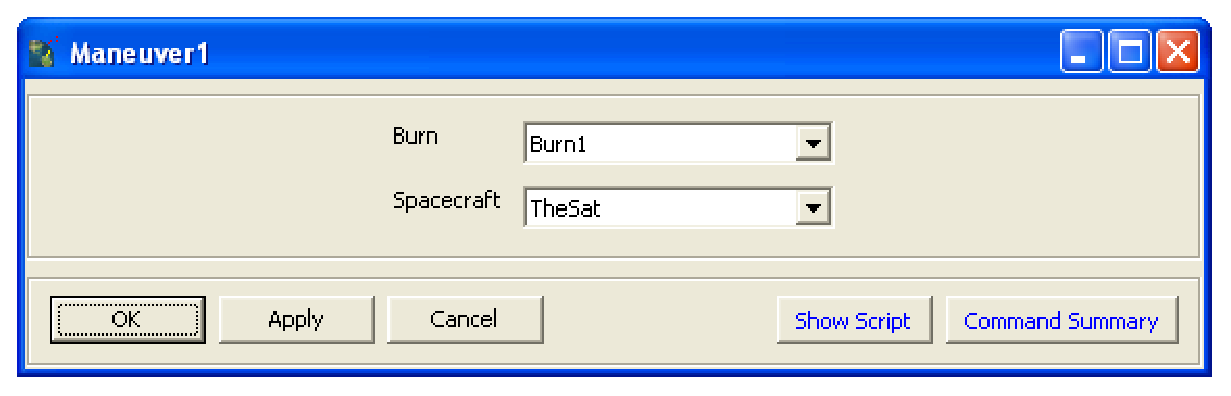
\includegraphics[scale=0.5]{Images/ManeuverPanel.eps}
\caption{\label{figure:ManeuverConfigPanel}The Maneuver Command Configuration Panel}
\end{center}
\end{figure}

The sequence diagram in Figure~\ref{figure:ManeuverConfiguration} shows the top level messages that
are passed when the Maneuver command is configured using this panel.  This view into the command
configuration includes a bit more detail about the GUI messages than was shown in the Spacecraft
configuration presented previously.

\begin{figure}[htb]
\begin{center}
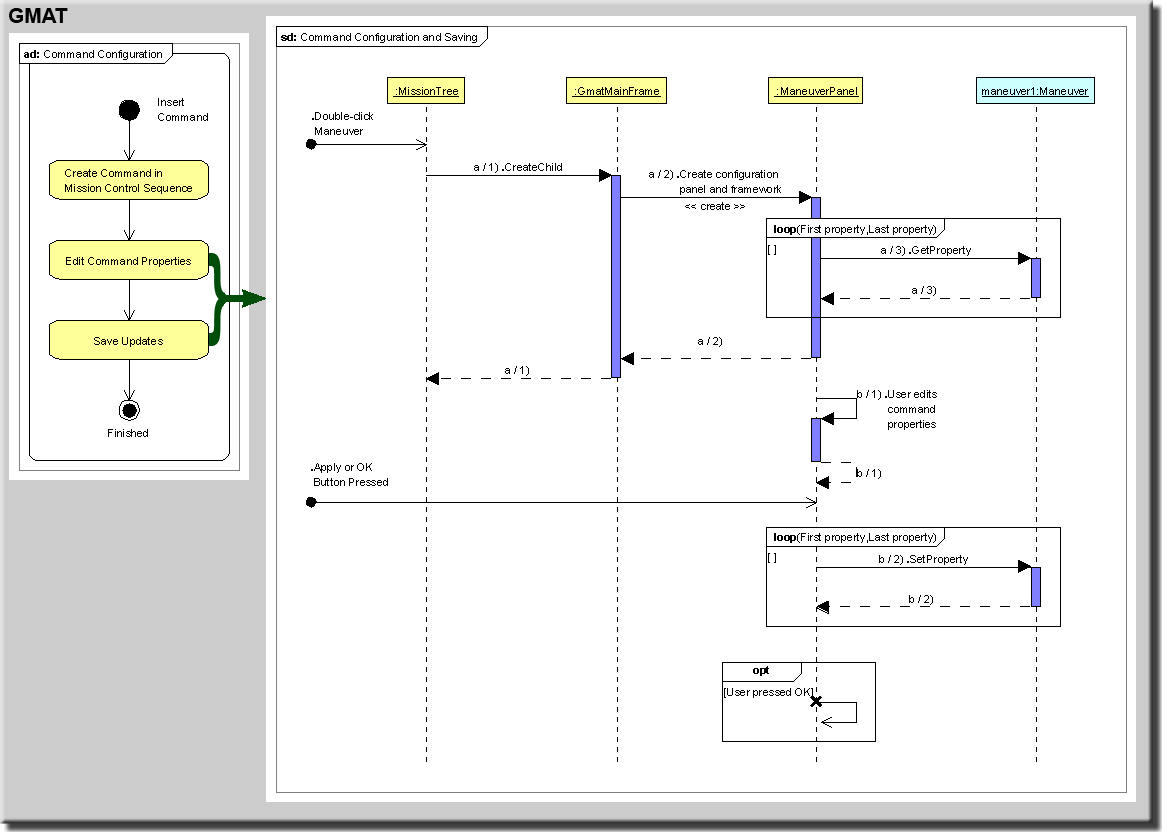
\includegraphics[scale=0.75]{Images/ManeuverConfiguration.eps}
\caption{\label{figure:ManeuverConfiguration}Command Configuration Example: Configuring the Maneuver
Command}
\end{center}
\end{figure}

The configuration process starts when the user double clicks on the command in the mission tree. 
The double click action sends a message to the MissionTree requesting the configuration panel for
the
selected node in the tree.  The MissionTree finds the item data, and sends that data to the main
GMAT window, called the GmatMainFrame, asking for a new child window configured to edit the
properties of the command contained in the item data.  The GmatMainFrame creates the child window
and displays it for the user.

More concretely, if the user double clicks on the Maneuver command created in the preceding
section, the tree item data for that maneuver command is passed from the MissionTree to the
GmatMainFrame.  The configuration window that should result from this action for display in the GUI
needs to contain the panel designed to match the underlying object that is being configured -- in
this case, a Maneuver command.  The GmatMainFrame uses the tree item data passed to it to determine
the type of panel needed by the child window during its creation. For this example, the
GmatMainFrame determines that the panel that is needed should be a ManeuverPanel because the tree
item data includes a pointer to a Maneuver command.  Accordingly, the GmatMainFrame creates an
instance of the ManeuverPanel class, and passes that panel to the child window.  The child window
receives the panel and places it into the corresponding container in the window.

Finally, the child window uses the command pointer in the tree item data to access the command and
determine the current values of its internal properties.  These data are collected from the command
and passed to the corresponding GUI components so that the user can see the current settings. Once
these data fields have been populated, the child window is displayed on the GUI, giving the GUI a
new window like that shown in Figure~{figure:ManeuverConfigPanel}.  This completes the top portion
of the sequence shown in Figure~\ref{figure:ManeuverConfiguration}.

Once the panel is shown on the GUI, the user makes changes to the settings for the command on the
new panel.  When the settings match the needs of the mission, the user clicks on either the ``OK''
or ``Apply'' button.  This action makes the ManeuverPanel update the Maneuver command with the new
settings.  If the user pressed the OK button, the child window also passes a message to GMAT
indicating that the user is finished with the window.  When that message is processed, the child
window is closed in the GUI.

\subsection{Model and Mission Persistence: Script Files}\index{Model!Scripts}

GMAT saves configuration data in files referred to as script files.  The details of the script file
parsing can be found in Chapter~\ref{chapter:ScriptRW}.  The following paragraphs provide an
overview of these processes.

The GMAT script files can be thought of as a serialized text view of the configured objects and
Mission Control Sequence constructed by the user to model spacecraft.  GMAT provides a subsystem,
controlled by the ScriptInterpreter, that manages reading and writing of these files.  All of these
script files are ASCII based files, so they can be edited directly by users.

\lstset{numbers=left}
\lstinputlisting[caption={A Basic GMAT Script File},label=listing:BasicScript,firstnumber=1]
{script/BasicScript.script}
\lstset{numbers=none}

Listing~\ref{listing:BasicScript} shows a simple script that propagates a spacecraft for
approximately 7~days, plotting the Cartesian components of the velocity against the spacecraft's X
coordinate value.  Details of all of these settings can be found in the User's
Guide\cite{userGuide}. This script just serves as an example for the discussion that follows.

All objects that are created as configured resources from the GUI are stored in the script files
using the keyword ``Create''.  In the script shown here, there are four resources: a Spacecraft
named ``sat1'', a ForceModel named ``fm'', a Propagator (actually an instance of the PropSetup
class) named ``prop'', and an XYPlot Subscriber named ``posvel''.  Each of these resources is used
when running the mission.

In GMAT, each resource can have one or more data members that users can set.  These resource
properties are initialized to default settings.  Users can override the values of these properties.
In the GUI, this action is performed by editing data presented on the panels for the resources.
Properties are changed in the script file by assigning new values to the properties by name; for
example, in the sample script, the Spacecraft's semimajor axis is changed to 10000.0 km on the fifth
line of script:

\begin{lstlisting}
sat1.SMA = 10000.0
\end{lstlisting}

\noindent The script shown here is a script as it might be entered by a user.  Only the lines that
override default property values are shown, and the lines are written as simply as possible.  The
full set of object properties can be examined by writing this object to a script file.  When a
Spacecraft -- or any other resource -- is saved, all of the resource properties are written.  In
addition, the keyword ``GMAT'' is written to the file, and the full precision data for the numerical
properties are written as well.  The Spacecraft configured in the script file above is written to
file as shown in Listing~\ref{listing:BasicMissionSpacecraft}.

\lstset{numbers=left,firstnumber=1}
\begin{lstlisting}[caption={Script Listing for a Spacecraft},label={listing:BasicMissionSpacecraft}]
Create Spacecraft sat1;
GMAT sat1.DateFormat = TAIModJulian;
GMAT sat1.Epoch = 21545.000000000;
GMAT sat1.CoordinateSystem = EarthMJ2000Eq;
GMAT sat1.DisplayStateType = Keplerian;
GMAT sat1.SMA = 9999.999999999998;
GMAT sat1.ECC = 0.2499999999999999;
GMAT sat1.INC = 78.5;
GMAT sat1.RAAN = 45;
GMAT sat1.AOP = 7.349999999999972;
GMAT sat1.TA = 0.9999999999999002;
GMAT sat1.DryMass = 850;
GMAT sat1.Cd = 2.2;
GMAT sat1.Cr = 1.8;
GMAT sat1.DragArea = 15;
GMAT sat1.SRPArea = 1;
\end{lstlisting}
\lstset{numbers=none}

\noindent GMAT generates the scripting for resources and commands using a method,
GetGeneratingString(), which is provided in the GmatBase class.  This class provides the
infrastructure needed to read and write object properties through a consistent set of interfaces.
The GetGeneratingString() method uses these interfaces when writing most user objects and commands
to script.  Derived classes can override the method as needed to write out class specific
information.
When GMAT saves a model to a script file, it tells the ScriptInterpreter to write a script file with
a given name.  The ScriptInterpreter systematically calls GetGeneratingString() on each object in
the configuration and sends the resulting serialized form of each object to the script file.  Once
all of the objects in the configuration have been saved, GMAT takes the first command in the Mission
Control Sequence and calls its GetGeneratingString() method, writing the resulting text to the
script file.  It traverses the command list, writing each command in sequential order.

Script reading inverts this process.  When a user tells GMAT to read a script, the name of the
script file is passed to the ScriptInterpreter.  The ScriptInterpreter then reads the file, one
logical block\footnote{A ``logical block'' of script is one or more lines of text sufficiently
detailed to describe a single action taken in GMAT.  Examples include creation of a resource,
setting of a single parameter on a resource, or adding a command to the Mission Control Sequence.}
at a time, and constructs and configures the scripted objects following a procedure similar to that
described above for actions taken from the GUI.

Details of script processing can be found in Chapter~\ref{chapter:ScriptRW}.

\subsection{\label{section:SandboxMCSExecution}Running a Mission}\index{Model!Running}

Once a user has configured a model in GMAT, the model is ready to be run.  The configuration has
been populated with all of the resources needed for the run, and the resources have been configured
to match the needs of the analyst.  The Mission Control Sequence has been entered and configured to
meet the needs of the mission.  All that remains is the actual running of the model encoded in these
elements.

Figure~\ref{figure:RunningBasicScript} shows the sequence followed when a mission is executed in
GMAT.  The figure shows the sequence as initiated in the GUI.  The user chooses to run the mission
by pressing the ``Run'' button on GMAT's toolbar.  This action sends a RunMission message to the
GuiInterpreter, which then calls the Moderator's RunMission() method (Step 1 in the figure).

The Moderator begins by clearing any stale data out of the Sandbox by calling the Sandbox's Clear()
method (Step 2).  This action removes any local copies of objects in the Sandbox that may still
exist from a previous run.  Once the Sandbox has been cleared, the Moderator begins passing
resources into the Sandbox.

The Moderator passes the current Solar System into the Sandbox, and then begins making calls to
ConfigurationManager to get the current set of resources used in the model (Step 3).  The Moderator
passes these resources into the Sandbox (Step 4) by type, starting with coordinate systems, and
proceeding until all of the resources have been passed into the Sandbox.  The Sandbox receives each
resource as it is passed in and makes a copy of that resource by calling its Clone() method (Steps 5
and 6).  The Sandbox stores these local clones by name in its local object map.  The local object
map contains the objects that are manipulated during a run; the configured objects are not used when
running the mission.

After the configured objects have been passed into the Sandbox, the Moderator sends the head node of
the Mission Control Sequence to the Sandbox\footnote{Commands are not cloned into the Sandbox at
this writing.  A future build of GMAT may require cloning of commands as well as resources, so that
the system can support multiple Sandboxes simultaneously.  The system is designed to allow this
extensibility when needed.} (Step 7).  This sets the Sandbox's internal sequence pointer to the
first command in the Mission Control Sequence (Step 8), completing steps needed to begin work in the
Sandbox.

\label{section:SandboxInitializationOverview}The Moderator has completed the bulk of its work for
the run at this point.  The next action taken is a call from the Moderator to the Sandbox,
instructing it to initialize itself (Step 9).  When the Sandbox receives this instruction, it begins
initializing the local objects.  Each object is queried for a list of referenced objects that need
to be set, and the Sandbox finds these objects in the local object store and sets each one on the
requesting object (Step 10, performed iteratively through all of the objects).  After the object
initialization, the Sandbox walks through the Mission Control Sequence node by node, passing each
command a pointer to the local object map and then calling the Command's Initialize method, giving
each command the opportunity to set up data structures needed to execute the Mission Control
Sequence  (Step 11, performed iteratively through the Mission Control Sequence).  If initialization
fails at any point during this process, the Sandbox halts the initialization process and reports the
error to the Moderator.

Once initialization is complete, the Sandbox reports successful initialization to the Moderator.  At
this point the Moderator sends an Execute() message to the Sandbox (Step 12).  The Sandbox responds
by calling the Execute() method on the first command in the Mission Control Sequence (Step 13).  The
command executes this method, manipulating objects in the local object map  (Step 14) and sending
data to GMAT's Publisher (Step 15) based on the design of each command.  When data is passed to the
Publisher, it passes the data on to each Subscriber (Step 16), producing output that the user can
view to monitor the mission as it executes, or to process after the mission has finished running.

When the first command completes execution, the Sandbox asks for the next node to execute in the
Mission Control Sequence, and repeats this process on the second node.  The process continues,
calling node after node in the Mission Control Sequence until the final command has been executed.

\begin{figure}[H]
\begin{center}
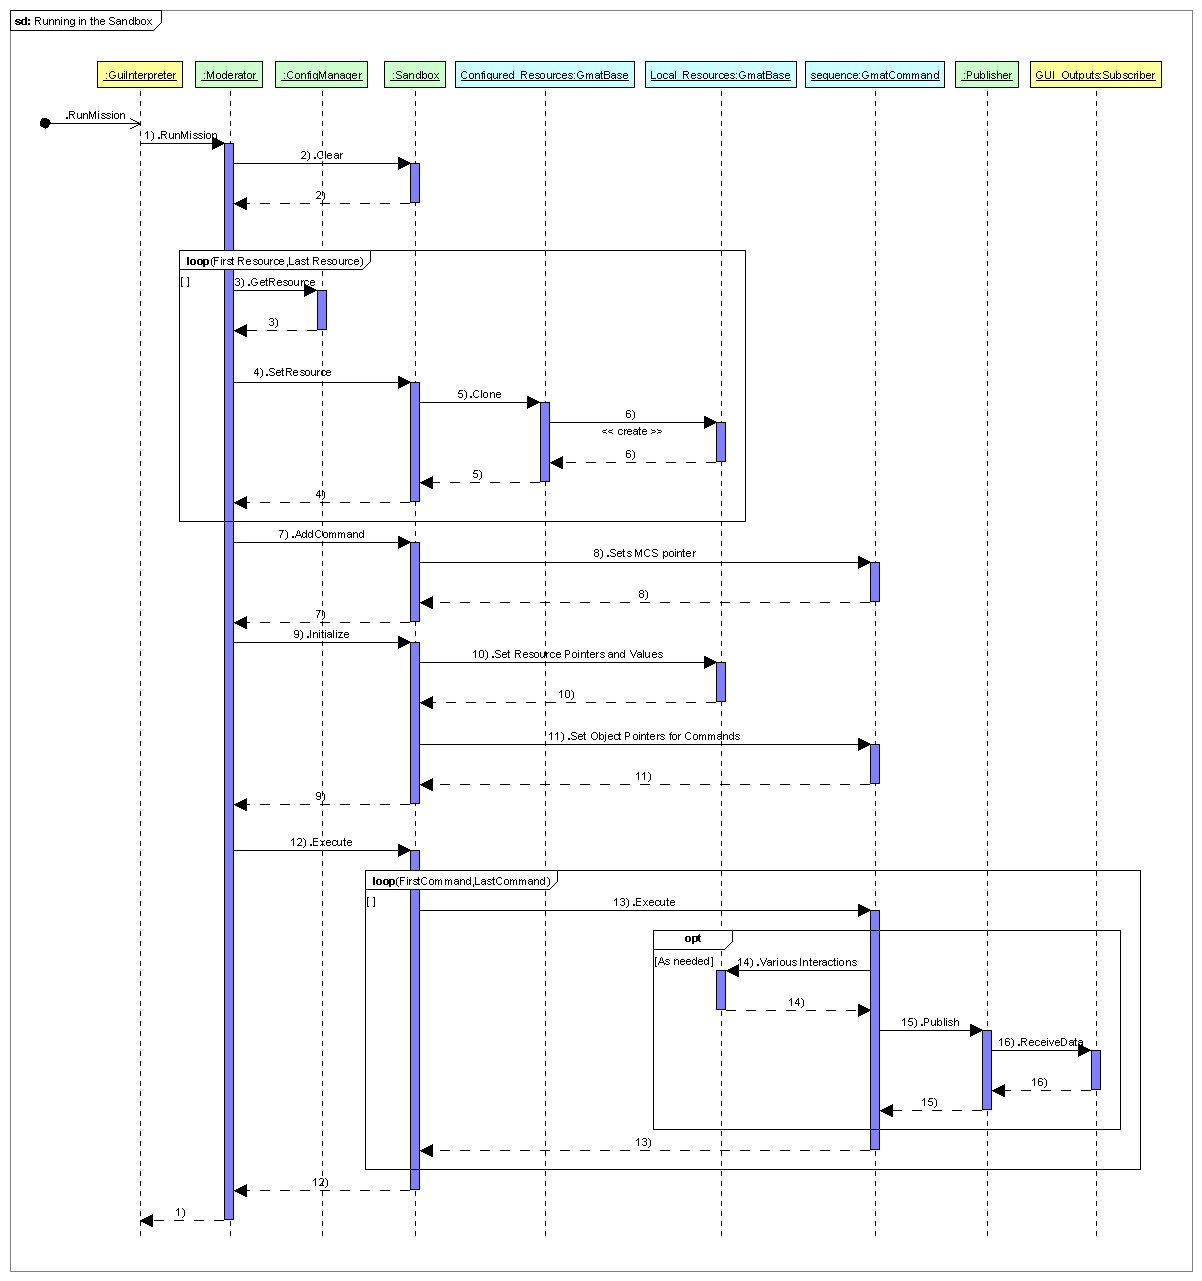
\includegraphics[scale=0.35]{Images/RunningintheSandbox.eps}
\caption{\label{figure:RunningBasicScript}The Sequence followed to Run a Mission}
\end{center}
\end{figure}

\begin{figure}[H]
\begin{center}
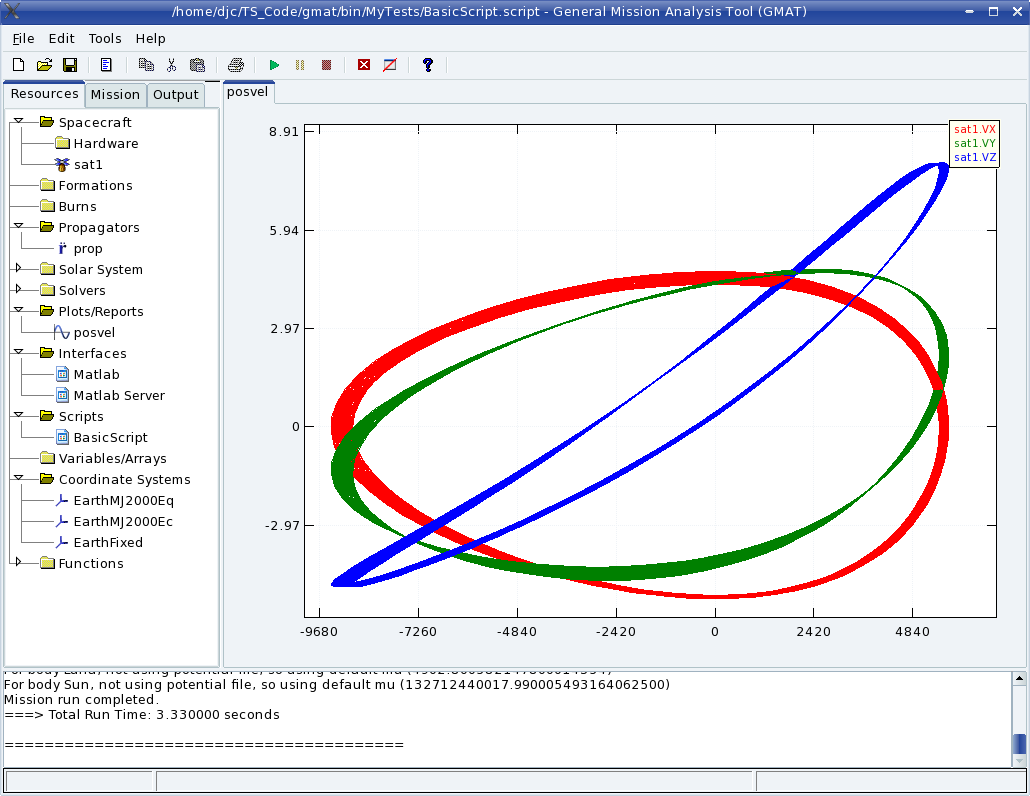
\includegraphics[scale=0.45]{Images/BasicMissionRunLinux.eps}%
\caption{\label{figure:BasicScriptOutput}Results of the Script Example, Run on Linux}%
\end{center}
\end{figure}

Once the final command has executed, the Sandbox sends a message to the Mission Control Sequence
stating that the run has completed execution, and control is returned to the Moderator from the
Sandbox.  The Moderator returns control to the GuiInterpreter, which returns control, through the
GUI, to the user, completing the mission run.  Figure~\ref{figure:BasicScriptOutput} shows the
results of this sequence when executed for the script shown in Listing~\ref{listing:BasicScript}.

\section{Summary}

This completes the presentation of the overview of GMAT's architecture.  In this chapter we have
discussed the basic architecture for GMAT, presented an overview of the arrangement of the
components of the system that we will build upon in upcoming chapters, and presented a programmatic
description of the workflow of three common tasks performed in GMAT: Starting the system, Creating
resources and comments for a spacecraft mission, and running that mission.

The next few chapters will present, in some detail, descriptions of each of the components of the
Engine package, followed by sections describing the infrastructure used for the Resources and
Commands, and then the design features of these elements.